% Copyright (C) 2010,2011,2012,2013,2014 The ESPResSo project
% Copyright (C) 2002,2003,2004,2005,2006,2007,2008,2009,2010 
%   Max-Planck-Institute for Polymer Research, Theory Group
%  
% This file is part of ESPResSo.
%   
% ESPResSo is free software: you can redistribute it and/or modify it
% under the terms of the GNU General Public License as published by the
% Free Software Foundation, either version 3 of the License, or (at your
% option) any later version.
%  
% ESPResSo is distributed in the hope that it will be useful, but
% WITHOUT ANY WARRANTY; without even the implied warranty of
% MERCHANTABILITY or FITNESS FOR A PARTICULAR PURPOSE.  See the GNU
% General Public License for more details.
%  
% You should have received a copy of the GNU General Public License
% along with this program.  If not, see <http://www.gnu.org/licenses/>.
%
\chapter{Setting up interactions}
\label{sec:inter}
\newescommand{inter}
\index{interactions|mainindex}

In \es, interactions are set up and investigated by the
\keyword{inter} command. There are mainly two types of interactions:
non-bonded and bonded interactions. Non-bonded interactions only
depend on the \emph{type} of the two involved particles. This also
applies to the electrostatic interaction; however, due to its
long-ranged nature, it requires special care and \es handles it
separately with a number of state-of-the-art algorithms. The particle
type and the charge are both defined using the \lit{part} command.

A bonded interaction defines an interaction between a number of
specific particles; it only applies to the set of particles for which
it has been explicitely set.  A bonded interaction between a set of
particles has to be specified explicitely by the \lit{part bond}
command, while the \lit{inter} command is used to define the
interaction parameters.

\begin{essyntax}
  inter
\end{essyntax}
Without any arguments, \lit{inter} returns a list of all defined
interactions as a Tcl-list. The format of each entry corresponds to
the syntax for defining the interaction as described below. Typically,
this list looks like
\begin{tclcode}
  {0 0 lennard-jones 1.0 2.0 1.1225 0.0 0.0} {0 FENE 7.0 2.0}
\end{tclcode}


\section{Isotropic non-bonded interactions}
\label{sec:inter-nb}
\index{Non-bonded interactions|mainindex}
\index{interactions!non-bonded|mainindex}

\begin{essyntax*}
  inter \var{type1} 
  \var{type2}
  \opt{\var{interaction}}
  \opt{\var{parameters}}
\end{essyntax*}
This command defines an interaction of type \var{interaction} between
all particles of type \var{type1} and \var{type2}. The possible
interaction types and their parameters are listed below. If the
interaction is omitted, the command returns the currently defined
interaction between the two types using the syntax to define the
interaction, \eg
\begin{tclcode}
  0 0 lennard-jones 1.0 2.0 1.1225 0.0 0.0
\end{tclcode}

For many non-bonded interactions, it is possible to artificially cap
the forces, which often allows to equilibrate the system much
faster. See the subsection~\ref{sec:forcecap} for details.


\subsection{Tabulated interaction}
\index{tabulated interaction|mainindex}
\index{interactions!tabulated|mainindex}
\label{sec:tabnonbonded}

\begin{essyntax}
  inter \var{type1} \var{type2} tabulated \var{filename}%
  \begin{features}
    \required{TABULATED}
  \end{features}
\end{essyntax}

This defines an interaction between particles of the types \var{type1} and
\var{type2} according to an arbitrary tabulated pair potential. \var{filename}
specifies a file which contains the tabulated forces and energies as a function
of the separation distance. The tabulated potential allows capping the force
using \lit{inter forcecap}, see section~\ref{sec:forcecap}.

At present the required file format is simply an ordered list separated by
whitespace. The data reader first looks for a {\tt \#} character and begins
reading from that point in the file. Anything before the {\tt \#} will be
ignored.

The first three parameters after the {\tt \#} specify the number of data points
$N_\mathrm{points}$ and the minimal and maximal tabulated separation distances
$r_\mathrm{min}$ and $r_\mathrm{max}$. The number of data points obviously should
be an integer, the two other can be arbitrary positive doubles. Take care when
choosing the number of points, since a copy of each lookup table is kept on each
node and must be referenced very frequently. The maximal tabulated separation
distance also acts as the effective cutoff value for the potential.

The remaining data in the file should consist of n data triples $r$, $F(r)$ and
$V(r)$. $r$ gives the particle separation, $V(r)$ specifies the interaction
potential, and $F(r)= -V'(r)/r$ the force (note the factor $1/r$!). The values
of $r$ are assumed to be equally distributed between $r_\mathrm{min}$ and
$r_\mathrm{max}$ with a fixed distance of
$(r_\mathrm{max}-r_\mathrm{min})/(N_\mathrm{points}-1)$; the distance values $r$ in
the file are ignored and only included for human readability.

\subsection{Lennard-Jones interaction}
\label{sec:LennardJones}

\index{Lennard-Jones interaction|mainindex}
\index{interactions!Lennard-Jones|mainindex}
\begin{essyntax}
  inter \var{type1} 
  \var{type2}
  lennard-jones 
  \var{\epsilon} \var{\sigma} 
  \var{r_\mathrm{cut}} 
  \opt{\alt{\var{c_\mathrm{shift}}|auto}
    \opt{\var{r_\mathrm{off}}
      \opt{\var{r_\mathrm{cap}} 
        \opt{ \var{r_\mathrm{min}}}}}}
  \begin{features}
    \required{LENNARD_JONES}
  \end{features}
\end{essyntax}

This command defines the traditional (12-6)-Lennard-Jones interaction
between particles of the types \var{type1} and \var{type2}.  The
potential is defined by
\begin{equation}
  \label{eq:lj}
  V_\mathrm{LJ}(r) = \Biggl\{
    \begin{array}{ll}
      4\epsilon((\frac{\var{\sigma}}{r-\var{r_\mathrm{off}}})^{12}
      - (\frac{\var{\sigma}}{r-\var{r_\mathrm{off}}})^6+\var{c_\mathrm{shift}}) 
      & \mathrm{, if~} \var{r_\mathrm{min}}+\var{r_\mathrm{off}} < \var{r} < \var{r_\mathrm{cut}}+\var{r_\mathrm{off}}\\
      \mathit{0} 
      & \mathrm{, otherwise}\\
    \end{array}.
\end{equation}

The traditional Lennard--Jones potential is the ``work--horse''
potential of particle--particle interactions in coarse--grained
simulations.  It is a simple model of the van--der--Waals interaction,
and is attractive at large distance, but strongly repulsive at short
distances.  $\var{r_\mathrm{off}} + \var{\sigma}$ corresponds to the
sum of the radii of the interaction particles; at this radius,
$V_\mathrm{LJ}(\var{r}) = 4 \var{\epsilon} \var{c_\mathrm{shift}}$.
The minimum of the potential is at $\var{r} = \var{r_\mathrm{off}} +
2^\frac{1}{6}\var{\sigma}$.  At this value of $r$, $V_\mathrm{LJ}(r) =
-\var{\epsilon} + 4 \var{\epsilon} \var{c_\mathrm{shift}}$. The
attractive part starts beyond this value of $\var{r}$.
$\var{r_\mathrm{cut}}$ determines the radius where the potential is
cut off. 

If \var{c_\mathrm{shift}} is not set or it is set to the string
\lit{auto}, the shift will be automatically computed such that the
potential is continuous at the cutoff radius. If \var{r_\mathrm{off}}
is not set, it is set to $0$.

The total force on a particle can be capped by using the command
\lit{inter forcecap}, see section~\ref{sec:forcecap}, or on an
individual level using the \var{r_\mathrm{cap}} variable. When
\var{r_\mathrm{cap}} is set \emph{and} \lit{inter forcecap
  individual} has been issued before, the maximal force that is generated by
this potential is the force at \var{r_\mathrm{cap}}.  By default,
force capping is off, \ie the cap radius is set to 0.

An optional additional parameter can be used to restrict the
interaction from a \emph{minimal} distance
$\var{r_\mathrm{min}}$. This is an optional parameter, set to 0 by
default.

A special case of the Lennard--Jones potential is the
Weeks--Chandler--Andersen (WCA) potential, which one obtains by
putting the cutoff into the minimum, \ie choosing
$\var{r_\mathrm{cut}}=2^\frac{1}{6}\var{\sigma}$. The WCA potential is
purely repulsive, and is often used to mimick hard sphere repulsion.


When coupling particles to a Shan-Chen fluid, if the \lit{affinity} interaction is set, the Lennard-Jones potential is multiplied by the function 

\begin{equation}
  \label{eq:lj-affinity}
  A(r) = \Biggl\{
    \begin{array}{ll}
      \frac{(1-\alpha_1)}{2} [1+\tanh(2\phi)]  +  \frac{(1-\alpha_2)}{2} [1+\tanh(-2\phi)]
      & \mathrm{, if~}  \var{r} > \var{r_\mathrm{cut}}+2^{\frac{1}{6}}\sigma\\
      1
      & \mathrm{, otherwise~} \\
    \end{array},
\end{equation}
where $\alpha_i$ is the affinity to the $i$-th fluid component (see
\ref{sec:affinity}), and the order parameter $\phi$ is calculated
from the fluid component local density as $\phi=\frac{\rho_1 -
\rho_2}{\rho_1+\rho_2}$. For example, if the affinities are chosen
so that the first component is a good solvent ($\alpha_1=1$) and
the second one is a bad solvent ($\alpha_2=0$), then, if the two
particles are both in a region rich in the first component, then
$\phi\simeq1$, and $A(r)\simeq0$ for
$r>\var{r_\mathrm{cut}}+2^{\frac{1}{6}}\sigma$.  Therefore, the
interaction potential will be very close to the WCA one. Conversely,
if both particles are in a region rich in the second component,
then $\phi\simeq-1$, and  $A(r)\simeq 1$, so that the potential
will be very close to the full LJ one. If the cutoff has been set
large enough, the particle will experience the attractive part of
the potential, mimiking the effective attraction induced by the bad
solvent.



\subsection{Generic Lennard-Jones interaction}
\index{Generic Lennard-Jones interaction|mainindex}
\index{interactions!Generic Lennard-Jones|mainindex}
\label{sec:GenLennardJones}

\begin{essyntax}
  inter \var{type1} 
  \var{type2}
  lj-gen
  \var{\epsilon} \var{\sigma} 
  \var{r_\mathrm{cut}} \var{c_\mathrm{shift}} \var{r_\mathrm{off}}
  \var{e_1} \var{e_2} \var{b_1} \var{b_2}
  \opt{\alt{\var{r_\mathrm{cap}}|auto} \var{\lambda} \var{\delta}}
  \begin{features}
    \required{LENNARD_JONES_GENERIC}
  \end{features}
\end{essyntax}

This command defines a generalized version of the Lennard-Jones
interaction (see section \ref{sec:LennardJones}) between particles of
the types \var{type1} and \var{type2}.  The potential is defined by
\begin{equation}
  \label{eq:lj-generic}
  V_\mathrm{LJ}(r) = \Biggl\{
    \begin{array}{ll}
      \epsilon(\var{b_1}(\frac{\var{\sigma}}{r-\var{r_\mathrm{off}}})^\var{e_1}
      -\var{b_2}(\frac{\var{\sigma}}{r-\var{r_\mathrm{off}}})^{e_2}+\var{c_\mathrm{shift}}) 
      & \mathrm{, if~} \var{r_\mathrm{min}}+\var{r_\mathrm{off}} < \var{r} < \var{r_\mathrm{cut}}+\var{r_\mathrm{off}}\\
      \mathit{0} 
      & \mathrm{, otherwise}\\
    \end{array}.
\end{equation}
Note that the prefactor 4 of the standard LJ potential is missing, so the normal
LJ potential is recovered for $b_1=b_2=4$, $e_1=12$ and $e_2=6$.

The total force on a particle can be capped by using the command
\lit{inter forcecap}, see section~\ref{sec:forcecap}, or on an
individual level using the \var{r_\mathrm{cap}} variable. When
\var{r_\mathrm{cap}} is set \emph{and} \lit{inter forcecap
  individual} has been issued before, the maximal force that is generated by
this potential is the force at \var{r_\mathrm{cap}}.  By default,
force capping is off, \ie the cap radius is set to 0.

The optional \texttt{LJGEN_SOFTCORE} feature activates a softcore version 
of the potential, where the following transformations apply: 
$\epsilon \rightarrow \lambda \epsilon$
and
$r-\var{r_\mathrm{off}} \rightarrow \sqrt{(r-\var{r_\mathrm{off}})^2 -
(1-\lambda) \delta \sigma^2}$. \var{\lambda} allows to tune the strength 
of the interaction, while \var{\delta} varies how smoothly the potential
goes to zero as $\var{\lambda}\rightarrow 0$. Such a feature allows one to
perform alchemical transformations, where a group of atoms can be slowly
turned on/off during a simulation.

\subsection{Lennard-Jones cosine interaction}
\index{Lennard-Jones cosine interaction|mainindex}
\index{interactions!Lennard-Jones cosine|mainindex}
\begin{essyntax}
  \variant{1}
  inter \var{type1} \var{type2} lj-cos
  \var{\epsilon} \var{\sigma}
  \var{r_\mathrm{cut}} \var{r_\mathrm{off}}
  \variant{2}
  inter \var{type1} \var{type2} lj-cos2
  \var{\epsilon} \var{\sigma} 
  \var{r_\mathrm{off}} \var{\omega}
  \begin{features}
    \required[\variant{1}]{LJCOS}
    \required[\variant{2}]{LJCOS2}
  \end{features}
\end{essyntax}
specifies a Lennard-Jones interaction with cosine
tail~\cite{soddeman01a} between particles of the types \var{type1} and
\var{type2}. The first variant behaves as follows: Until the minimum
of the Lennard-Jones potential at $\var{r_\mathrm{min}} = r_\mathrm{off} +
2^{\frac{1}{6}}\sigma$, it behaves identical to the unshifted
Lennard-Jones potential ($\var{c_\mathrm{shift}}=0$).  Between
\var{r_\mathrm{min}} and \var{r_\mathrm{cut}}, a cosine is used to
smoothly connect the potential to 0, \ie
\begin{equation}
  V(r)=\frac{1}{2}\epsilon\left(cos\left[\alpha(\var{r}-\var{r_\mathrm{off}})^2 + \beta\right]-1\right),
\end{equation}
where
$\alpha = \pi\left[(\var{r_\mathrm{cut}}-\var{r_\mathrm{off}})^2-(\var{r_\mathrm{min}}-\var{r_\mathrm{off}})^2\right]^{-1}$
and
$\beta = \pi - \left(\var{r_\mathrm{min}}-\var{r_\mathrm{off}}\right)^2\alpha$.

In the second variant, the cutoff radius is
$\var{r_\mathrm{cut}}=\var{r_\mathrm{min}} + \omega$, where $\var{r_\mathrm{min}} =  r_\mathrm{off} +
2^{\frac{1}{6}}\sigma$ as in the first variant. The potential
between $\var{r_\mathrm{min}}$ and $\var{r_\mathrm{cut}}$ is given by
\begin{equation}
  V(r)=\epsilon\cos^2\left[\frac{\pi}{2\omega}(\var{r} - \var{r_\mathrm{min}})\right].
\end{equation}
For $\var{r} < \var{r_\mathrm{min}}$, $V(r)$ is implemented as normal
Lennard-Jones potential, see equation \ref{eq:lj} with
$\var{c_\mathrm{shift}} = 0$.

Only the second variant allows capping the force using \lit{inter
  forcecap}, see section~\ref{sec:forcecap}.

\subsection{Smooth step interaction}
\index{smooth-step interaction|mainindex}
\index{interactions!smooth-step|mainindex}
\begin{essyntax}
  inter \var{type1} \var{type2}
  smooth-step \var{\sigma_1} \var{n} \var{\epsilon} \var{k_0}
  \var{\sigma_2} \var{r_\mathrm{cut}}
  \begin{features}
    \required{SMOOTH_STEP}
  \end{features}
\end{essyntax}
This defines a smooth step interaction between particles of the
types \var{type1} and \var{type2}, for which the potential is
\begin{equation}
  V(r)= \left(\var{\sigma_1}/d\right)^\var{n} + \epsilon/(1 + \exp\left[2k_0 (r - \sigma_2)\right])
\end{equation}
for $r<r_\mathrm{\var{cut}}$, and $V(r)=0$ elsewhere. With $n$ around
10, the first term creates a short range repulsion similar to the
Lennard-Jones potential, while the second term provides a much softer
repulsion. This potential therefore introduces two length scales, the
range of the first term, $\sigma_1$, and the range of the second one,
$\sigma_2$, where in general $\sigma_1<\sigma_2$.

\subsection{BMHTF potential}
\index{BMHTF interaction|mainindex}
\index{interactions!BMHTF|mainindex}
\begin{essyntax}
  inter \var{type1} \var{type2}
  bmhtf-nacl \var{A} \var{B} \var{C} \var{D} \var{\sigma} \var{r_\mathrm{cut}}
  \begin{features}
    \required{BMHTF_NACL}
  \end{features}
\end{essyntax}
This defines an interaction with the {\em short-ranged part} of the
Born-Meyer-Huggins-Tosi-Fumi potential between particles of the types
\var{type1} and \var{type2}, which is often used to simulate NaCl
crystals. The potential is defined by:
\begin{equation}
  V(r)= \var{A}\exp\left[\var{B}(\var{\sigma} - \var{r})\right] -
  \var{C} \var{r}^{-6} - \var{D} \var{r}^{-8} + \epsilon_\mathrm{shift},
\end{equation}
where $\epsilon_\mathrm{shift}$ is chosen such that
$V(\var{r_\mathrm{cut}})=0$. For $r\ge \var{r_\mathrm{cut}}$, the
$V(r)=0$.

For NaCl, the parameters should be chosen as follows:

\begin{tabular}{r|l|l|l|l|l}
  types & \var{A} (\unitfrac{kJ}{mol}) & \var{B} ($\unit{\AA^{-1}}$) &
  \var{C} ($\unit{\AA^6}$\unitfrac{kJ}{mol}) & \var{D}
  $\unit{\AA^8}$\unitfrac{kJ}{mol} & \var{\sigma} (\unit{\AA}) \\
  \hline
  Na-Na & 25.4435 & 3.1546 &  101.1719 &    48.1771 & 2.34 \\
  Na-Cl & 20.3548 & 3.1546 &  674.4793 &   837.0770 & 2.755 \\
  Cl-Cl & 15.2661 & 3.1546 & 6985.6786 & 14031.5785 & 3.170 \\
\end{tabular}

The cutoff can be chosen relatively freely because the potential
decays fast; a value around 10 seems reasonable.

In addition to this short ranged interaction, one needs to add a
Coulombic, long--ranged part. If one uses elementary charges, \ie a
charge of $q=+1$ for the Na--particles, and $q=-1$ for the
Cl--particles, the corresponding prefactor of the Coulomb interaction
is $\approx 1389.3549 \AA\,kJ/mol$.

\subsection{Morse interaction}
\index{Morse interaction|mainindex}
\index{interactions!Morse|mainindex}

\begin{essyntax}
  inter \var{type1} \var{type2} morse
  \var{\epsilon} \var{\alpha} \var{r_\mathrm{min}} \var{r_\mathrm{cut}}
  \begin{features}
    \required{MORSE}
  \end{features}
\end{essyntax}
This defines an interaction using the Morse potential between
particles of the types \var{type1} and \var{type2}. It serves similar
purposes as the Lennard-Jones potential, but has a deeper minimum,
around which it is harmonic.  This models the potential energy in a
diatomic molecule.  This potential allows capping the force using
\texttt{inter forcecap}, see section~\ref{sec:forcecap}.

For $r < \var{r_\mathrm{cut}}$, this potential is given by
\begin{equation}
  V(r)=\var{\epsilon}\left(\exp\left[-2 \var{\alpha} \left(r - \var{r_\mathrm{min}}\right)\right]
    - 2\exp\left[-\alpha\left(r - r_\mathrm{min}\right)\right]\right) -
  \epsilon_\mathrm{shift},
\end{equation}
where \var{\epsilon_\mathrm{shift}} is again chosen such that
$V(\var{r_\mathrm{cut}})=0$. For $r\ge \var{r_\mathrm{cut}}$, the $V(r)=0$.

\subsection{Buckingham interaction}
\index{Buckingham interaction|mainindex}
\index{interactions!Buckingham|mainindex}

\begin{essyntax}
  inter \var{type1} \var{type2} buckingham
  \var{A} \var{B} \var{C} \var{D}
  \var{r_\mathrm{cut}} \var{r_\mathrm{discont}} \var{\epsilon_\mathrm{shift}}
  \begin{features}
    \required{BUCKINGHAM}
  \end{features}
\end{essyntax}
This defines a Buckingham interaction between particles of the types
\var{type1} and \var{type2}, for which the potential is given by
\begin{equation}
  V(r)= A\exp(-B r) - Cr^{-6} - Dr^{-4} + \var{\epsilon_\mathrm{shift}}
\end{equation}
for $\var{r_\mathrm{discont}} < r < \var{r_\mathrm{cut}}$. Below \var{r_\mathrm{discont}},
the potential is linearly continued towards $r=0$, similarly to force capping,
see below. Above $r=\var{r_\mathrm{cut}}$, the potential is $0$. This potential
allows capping the force using \lit{inter forcecap}, see
section~\ref{sec:forcecap}.

\subsection{Soft-sphere interaction}
\index{soft-sphere interaction|mainindex}
\index{interactions!soft-sphere|mainindex}

\begin{essyntax}
  inter \var{type1} \var{type2}
  soft-sphere \var{a} \var{n} \var{r_\mathrm{cut}} \var{r_\mathrm{offset}}
  \begin{features}
    \required{SOFT_SPHERE}
  \end{features}
\end{essyntax}
This defines a soft sphere interaction between particles of the types
\var{type1} and \var{type2}, which is defined by a single power law:
\begin{equation}
  V(r)=a\left(r-r_\mathrm{\var{offset}}\right)^{-n}
\end{equation}
for $r<\var{r_\mathrm{cut}}$, and $V(r)=0$ above. There is no shift
implemented currently, which means that the potential is discontinuous
at $r=\var{r_\mathrm{cut}}$. Therefore energy calculations should be
used with great caution.

\subsection{Hat interaction}
\index{hat interaction|mainindex}
\index{interactions!hat|mainindex}

\begin{essyntax}
  inter \var{type1} \var{type2}
  hat \var{F_\text{max}} \var{r_c}
  \begin{features}
    \required{HAT}
  \end{features}
\end{essyntax}
This defines a simple force ramp between particles of the types \var{type1} and
 \var{type2}. The maximal force \var{F_\text{max}} acts at zero distance and 
zero force is applied at distances $r_c$ and bigger. For distances smaller than 
\var{r_c}, the force is given by
\begin{equation}
  F(r)=F_{\text{max}} \cdot \left( 1 - \frac{r}{r_c} \right),
\end{equation}
for distances exceeding \var{r_c}, the force is zero.

The potential energy is given by
\begin{equation}
  V(r)=F_{\text{max}} \cdot (r-r_c) \cdot \left( \frac{r+r_c}{2r_c} - 1 \right),
\end{equation}
which is zero for distances bigger than \var{r_c} and continuous at distance 
\var{r_c}.

This is the standard conservative DPD potential and can be used in combination 
with \lit{inter DPD} \ref{sec:DPDinter}. The potential is also useful for live 
demonstrations, where a big time step may be employed to obtain quick results
on a weak machine, for which the physics do not need to be entirely correct.  

\subsection{Hertzian interaction}
\index{Hertzian interaction|mainindex}
\index{interactions!hertzian|mainindex}

\begin{essyntax}
  inter \var{type1} \var{type2}
  hertzian \var{\sigma} \var{\epsilon}
  \begin{features}
    \required{HERTZIAN}
  \end{features}
\end{essyntax}
This defines an interaction according to the Hertzian potential
between particles of the types \var{type1} and \var{type2}. The
Hertzian potential is defined by
\begin{equation}
  V(r)=
  \begin{cases} \epsilon\left(1-\frac{r}{\sigma}\right)^{5/2} & r < \sigma\\
    0 & r \ge \sigma.
  \end{cases}
\end{equation}
The potential has no singularity and is defined everywhere; the
potential has nondifferentiable maximum at $r=0$, where the force is
undefined.

\subsection{Gaussian}
\index{Gaussian interaction|mainindex}
\index{interactions!gaussian|mainindex}

\begin{essyntax}
  inter \var{type1} \var{type2}
  gaussian \var{\sigma} \var{\epsilon} \var{r_\mathrm{cut}}
  \begin{features}
    \required{GAUSSIAN}
  \end{features}
\end{essyntax}
This defines an interaction according to the Gaussian potential 
between particles of the typers \var{type1} and \var{type2}.  The
Gaussian potential is defined by
\begin{equation}
  V(r) = 
  \begin{cases} \epsilon\,e^{-\frac{1}{2}\left(\frac{r}{\sigma}\right)^{2}}
    & r < \var{r_\mathrm{cut}}\\
  0 & r \ge \var{r_\mathrm{cut}}
  \end{cases}
\end{equation}
The Gaussian potential is smooth except at the cutoff, and has a
finite overlap energy of $\epsilon$. It can be used to model \eg{}
overlapping polymer coils. 

Currently, there is no shift implemented, which means that the potential 
is discontinuous at $r=\var{r_\mathrm{cut}}$.  Therefore use caution when 
performing energy calculations. However, you can often choose the
cutoff such that the energy difference at the cutoff is less than a
desired accuracy, since the potential decays very
rapidly.

\section{Anisotropic non-bonded interactions}
\label{inter-anisotropic}
\index{Anisotropic interactions}

\subsection{Directional Lennard-Jones interaction}
\index{Directional Lennard-Jones interaction|mainindex}
\index{interactions!Directional Lennard-Jones|mainindex}
\begin{essyntax}
  inter \var{type1} \var{type2} lj-angle
  \var{\epsilon} \var{\sigma}
  \var{r_\mathrm{cut}} \var{b1_a} \var{b1_b}
  \var{b2_a} \var{b2_b} \opt{\var{r_\mathrm{cap}} 
    \var{z_0} \var{\delta z} \var{\kappa} \var{\epsilon'}}
  \begin{features}
    \required{LJ_ANGLE}
  \end{features}
\end{essyntax}

\begin{center}
  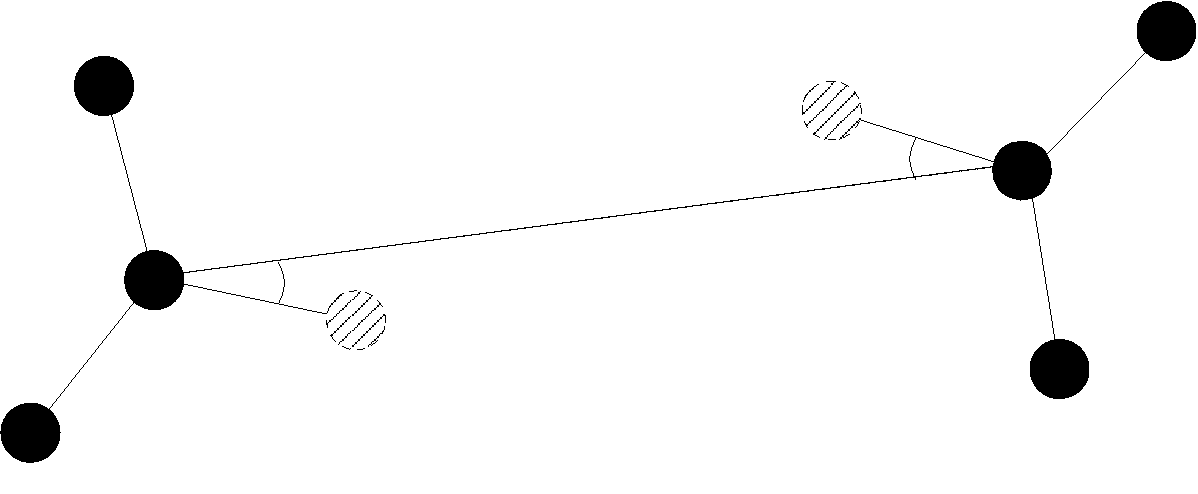
\includegraphics[height=8em]{figures/hbond}
\end{center}

Specifies a 12-10 Lennard-Jones interaction with angular dependence between
particles of the types \var{type1} and \var{type2}. These two particles need
two bonded partners oriented in a symmetric way. They define an orientation
for the central particle. The purpose of using bonded partners is to avoid
dealing with torques, therefore the interaction does \emph{not} need the
ROTATION feature. The angular part of the potential minimizes the system when
the two central beads are oriented along the vector formed by these two
particles. The shaded beads on the image are virtual particles that are formed
from the orientation of the bonded partners, connected to the central
beads. They are used to define angles. The potential is of the form
\begin{equation}
  U(r_{ik},\theta_{jik},\theta_{ikn})=
  \epsilon\left[5\left(\frac{\sigma}r\right)^{12} - 
    6\left(\frac{\sigma}{r}\right)^{10}\right]
  \cos^2\theta_{jik}\cos^2\theta_{ikn},
\end{equation}
where $r_{ik}$ is the distance between the two central beads, and each angle
defines the orientation between the direction of a central bead (determined
from the two bonded partners) and the vector $\mathbf{r_{ik}}$. Note that the
potential is turned off if one of the angle is more than $\pi/2$. This way we
don't end up creating a minimum for an anti-parallel configuration.

Unfortunately, the bonded partners are not seeked dynamically. One has to keep
track of the relative positions of the particle IDs. This can be done by
setting the parameters \var{b1_a}, \var{b1_b}, \var{b2_a}, and \var{b2_b}. Say
the first bead \var{type1} has particle ID \var{n}, then one should set the
simulation such as its two bonded partners have particle IDs \var{n+b1_a} and
\var{n+b1_b}, respectively. On a linear chain, for example, one would
typically have \var{b1_a=1} and \var{b1_b=-1} such that the central bead and
its two bonded partners have position IDs \var{n}, \var{n+1}, and \var{n-1},
respectively. This is surely not optimized, but once the simulation is set
correctly the algorithm is very fast.

The force can be capped using \lit{inter forcecap}. It might turn out
to be useful in some cases to keep this capping during the whole
simulation. This is due to the very sharp angular dependence for small
distance, compared to $\sigma$. Two beads might come very close to each other
while having unfavorable angles such that the interaction is turned off. Then
a change in the angle might suddenly turn on the interaction and the system
will blow up (the potential is so steep that one would need extremely small
time steps to deal with it, which is not very clever for such rare events).

For instance, when modeling hydrogen bonds (N-H...O=C), one can avoid
simulating hydrogens and oxygens by using this potential. This comes down to
implementing a HBond potential between N and C atoms.

The optional parameter \var{r_\mathrm{cap}} is the usual cap radius. The four
other optional parameters (\var{z_0}, \var{\delta z}, \var{\kappa},
\var{\epsilon'}) describe a different interaction strength \var{\epsilon'} for
a subset of the simulation box. The box is divided through the \var{z} plane
in two different regions: region 1 which creates an interaction with strength
\var{\epsilon}, region 2 with interaction strength \var{\epsilon'}. The 2nd
region is defined by its \var{z}-midplane \var{z_0}, its total thickness
\var{\delta z}, and the interface width \var{\kappa}. Therefore, the
interaction strength is \var{\epsilon} everywhere except for the region of the
box $z_0-\delta z/2<z<z_0+\delta z/2$. The interface width smoothly
interpolates between the two regions to avoid discontinuities. As an example,
one can think of modeling hydrogen bonds in two different environments: water,
where the interaction is rather weak, and in a lipid bilayer, where it is
comparatively stronger.

\subsection{Gay-Berne interaction}
\index{Gay-Berne interaction|mainindex}
\index{interactions!Gay-Berne|mainindex}

\begin{essyntax}
  inter \var{type1} \var{type2} gay-berne
  \var{\epsilon_0} \var{\sigma_0} \var{r_\mathrm{cutoff}}
  \var{k1} \var{k2} \var{\mu} \var{\nu}
  \begin{features}
    \required{ROTATION}
    \required{GAY_BERNE}
  \end{features}
\end{essyntax}
This defines a Gay-Berne potential for prolate and oblate particles
between particles of the types \var{type1} and \var{type2}. The
Gay-Berne potential is an anisotropic version of the classic
Lennard-Jones potential, with orientational dependence of the range
\var{\sigma_0} and the well-depth \var{\epsilon_0}.

Assume two particles with orientations given by the unit vectors
$\mathbf{\hat{u}}_i$ and $\mathbf{\hat{u}}_j$ and intermolecular vector
$\mathbf{r} = r\mathbf{\hat{r}}$. If $r<r_\mathrm{\var{cut}}$, then the
interaction between these two particles is given by
\begin{equation}
  V(\mathbf{r}_{ij}, \mathbf{\hat{u}}_i, \mathbf{\hat{u}}_j) = 4
  \epsilon(\mathbf{\hat{r}}_{ij}, \mathbf{\hat{u}}_i,
  \mathbf{\hat{u}}_j) \left( \tilde{r}_{ij}^{-12}-\tilde{r}_{ij}^{-6}
  \right),
\end{equation}
otherwise $V(r)=0$. The reduced radius is
\begin{equation}
  \tilde{r}=\frac{r - \sigma(\mathbf{\hat{r}},
    \mathbf{\hat{u}}_i, \mathbf{\hat{u}}_j)+\sigma_0}{\sigma_0},
\end{equation}
\begin{equation}
  \sigma( \mathbf{\hat{r}}, \mathbf{\hat{u}}_i,
  \mathbf{\hat{u}}_j) = \sigma_{0} \left\{ 1 - \frac{1}{2} \chi \left[
      \frac{ \left( \mathbf{\hat{r}} \cdot \mathbf{\hat{u}}_i +
          \mathbf{\hat{r}} \cdot \mathbf{\hat{u}}_j \right)^{2} }
      {1 + \chi \mathbf{\hat{u}}_i \cdot \mathbf{\hat{u}}_j } +
      \frac{ \left( \mathbf{\hat{r}} \cdot \mathbf{\hat{u}}_i -
          \mathbf{\hat{r}} \cdot \mathbf{\hat{u}}_j \right)^{2} }
      {1 - \chi \mathbf{\hat{u}}_i \cdot \mathbf{\hat{u}}_j}
    \right] \right\}^{-\frac{1}{2}}
\end{equation}
and
\begin{multline}
  \epsilon(\mathbf{\hat{r}}, \mathbf{\hat{u}}_i,
  \mathbf{\hat{u}}_j) = \\
  \epsilon_0 \left( 1- \chi^{2}(\mathbf{\hat{u}}_i
    \cdot \mathbf{\hat{u}}_j) \right)^{-\frac {\nu}{2}} \left[1-\frac
    {\chi'}{2} \left( \frac { (\mathbf{\hat{r}} \cdot
        \mathbf{\hat{u}}_i+ \mathbf{\hat{r}} \cdot
        \mathbf{\hat{u}}_j)^{2}} {1+\chi' \, \mathbf{\hat{u}}_i \cdot
        \mathbf{\hat{u}}_j }+ \frac {(\mathbf{\hat{r}} \cdot
        \mathbf{\hat{u}}_i-\mathbf{\hat{r}} \cdot
        \mathbf{\hat{u}}_j)^{2}} {1-\chi' \, \mathbf{\hat{u}}_i \cdot
        \mathbf{\hat{u}}_j } \right) \right]^{\mu}.
\end{multline}
The parameters $\chi = \left(k_1^{2} - 1\right)/\left(k_1^{2} +
  1\right)$ and $\chi' = \left(k_2^{1/\mu} -
  1\right)/\left(k_2^{1/\mu} + 1\right)$ are responsible for the
degree of anisotropy of the molecular properties.  \var{k_1} is the
molecular elongation, and \var{k_2} is the ratio of the potential well
depths for the side-by-side and end-to-end configurations.  The
exponents \var{\mu} and \var{\nu} are adjustable parameters of the
potential.  Several Gay-Berne parametrizations exist, the original one
being $\var{k_1} = 3$, $\var{k_2} = 5$, $\var{\mu} = 2$ and $\var{\nu}
= 1$.

\subsection{Affinity interaction}
\label{sec:affinity}

\index{Affinity interaction|mainindex}
\index{interactions!Affinity|mainindex}
\begin{essyntax}
  inter \var{type1} 
  \var{type2}
  affinity
  \var{\alpha_1} \var{\alpha_2} 
  \begin{features}
    \required{SHANCHEN}
  \end{features}
\end{essyntax}

Instead of defining a new interaction, this command acts as a
modifier for existing interactions, so that the conditions of
good/bad solvent associated to the two components of a Shan-Chen
fluid. The two types must match those of the interaction that one
wants to modify, and the two affinity values \var{\alpha_1} and
\var{\alpha_2} are values between 0 and 1. A value of 1 (of 0)
indicates that the component acts as a good (bad) solvent. The
specific functional form depends on the interaction type and is
listed in the interaction section.  So far, only the standard
Lennard-Jones interaction is modified by the \lit{affinity}
interaction.



\section{Bonded interactions}
\label{sec:inter-bonded}
\index{bonded interactions|mainindex}
\index{interactions!bonded|mainindex}

\begin{essyntax*}
  inter \var{bondid}
  \opt{\var{interaction}}
  \opt{\var{parameters}}
\end{essyntax*}

\index{bonded interaction type id} Bonded interactions are identified
by their \emph{bonded interaction type identificator} \var{bondid},
which is a non-negative integer.  The \lit{inter} \var{bondid} command
is used to specify the type and parameters of a bonded interaction,
which applies to all particles connected explicitely by this bond
using the \keyword{part} command (see section \vref{tcl:part}).
Therefore, defining a bond between two particles always involves two
steps: defining the interaction and applying it. Assuming that two
particles with ids 42 and 43 already exist, one can create \eg a
FENE-bond between them using
\begin{tclcode}
  inter 1 fene 10.0 2.0
  part 42 bond 1 43
\end{tclcode}
If a FENE-bond with the same interaction parameters is required between several
particles (\eg in a simple chain molecule), one can use the sampe type \var{id}:
\begin{tclcode}
  inter 1 fene 10.0 2.0
  part 42 bond 1 43; part 43 bond 1 44 
\end{tclcode}

Bonds can have more than just two bond partners. For the \keyword{inter} command
that does not play a role as it only specifies the parameters, only when
applying the bond using the \keyword{bond} particle, the number of involved
particles plays a role. The number of involved particles and their order, if
important, is nevertheless specified here for completeness.

\subsection{FENE bond}
\index{FENE bond|mainindex}
\index{interactions!FENE|mainindex}

\begin{essyntax}
  inter \var{bondid}
  fene
  \var{K} \var{\Delta r_\mathrm{max}} \opt{\var{r_0}}
\end{essyntax}
This creates a bond type with identificator \var{bondid} with a
FENE (finite extension nonlinear expander) interaction. This is a
rubber-band-like, symmetric interaction betweeen two particles with
prefactor \var{K}, maximal stretching \var{\Delta r_\mathrm{max}} and
equilibrium bond length \var{r_0}.  The bond potential diverges at a
particle distance $r=\var{r_0}-\var{\Delta r_\mathrm{max}}$ and
$r=\var{r_0}+\var{\Delta r_\mathrm{max}}$. It is given by
\begin{equation}
  V(r) = -\frac{1}{2} \var{K} \var{\Delta r_\mathrm{max}}^2\ln \left[ 1 - \left(
      \frac{r-\var{r_0}}{\var{\Delta r_\mathrm{max}}} \right)^2 \right].
\end{equation}

\subsection{Harmonic bond}
\index{harmonic bond|mainindex}
\index{interactions!harmonic|mainindex}

\begin{essyntax}
  inter \var{bondid}
  harmonic \var{K} \var{R} \opt{\var{r_\mathrm{cut}}}
\end{essyntax}
This creates a bond type with identificator \var{bondid} with a
classical harmonic potential. It is a symmetric interaction between two
particles. The potential is minimal at particle distance $r=R$, and the
prefactor is $K$. It is given by
\begin{equation}
  V(r) = \frac{1}{2} K \left( r - R \right)^2
\end{equation}
The third, optional parameter \var{r_\mathrm{cut}} defines a cutoff
radius.  Whenever a harmonic bond gets longer than
\var{r_\mathrm{cut}}, the bond will be reported as broken, and a
background error will be raised.

\subsection{Subtracted Lennard-Jones bond}
\index{subtracted Lennard-Jones bond|mainindex}
\index{interactions!subtracted Lennard-Jones|mainindex}

\begin{essyntax}
  inter \var{bondid}
  subt_lj
  \var{reserved} \var{R}
\end{essyntax}
This creates a ``bond'' type with identificator \var{bondid}, which
acts between two particles and actually subtracts the Lennard-Jones interaction
between the involved particles.  The first parameter, \var{reserved} is a dummy
just kept for compatibility reasons. The second parameter, \var{R}, is used as a
check: if any bond length in the system exceeds this value, the program
terminates. When using this interaction, it is worthwhile to consider
capping the Lennard-Jones potential appropriately so that round-off errors can
be avoided.

This interaction is useful when using other bond potentials which already
include the short--ranged repulsion. This often the case for force fields or in
general tabulated potentials.

\subsection{Rigid bonds}
\index{rigid bond|mainindex}
\index{interactions!rigid bond|mainindex}
\index{Rattle Shake algorithm}
\label{sec:rattle}

\begin{essyntax}
  inter \var{bondid}
  rigid_bond
  \var{constrained\_bond\_distance} \var{positional\_tolerance} 
  \var{velocity\_tolerance}
\end{essyntax}

To simulate rigid bonds, \es uses the Rattle Shake algorithm which
satisfies internal constraints for molecular models with internal
constraints, using Lagrange multipliers.\cite{andersen83a}

\subsection{Tabulated bond interactions}
\index{tabulated bond interactions|mainindex}
\index{interactions!tabulated bond|mainindex}

\begin{essyntax}
    \variant{1} inter \var{bondid}
    tabulated bond \var{filename}
    \variant{2} inter \var{bondid}
    tabulated angle \var{filename}
    \variant{3} inter \var{bondid}
    tabulated dihedral \var{filename}
\end{essyntax}

This creates a bond type with identificator \var{bondid} with a
two-body bond length (variant \variant{1}), three-body angle (variant
\variant{2}) or four-body dihedral (variant \variant{3}) tabulated
potential. The tabulated forces and energies have to be provided in a
file \var{filename}, which is formatted identically as the files for
non-bonded tabulated potentials (see section \ref{sec:tabnonbonded}).

The potential is calculated as follows:
\begin{itemize}
\item Variant~\variant{1} is a two body interaction depending on the distance of
  two particles. The force acts in the direction of the connecting vector
  between the particles. The bond breaks above the tabulated range, but for
  distances smaller than the tabulated range, a linear extrapolation based on
  the first two tabulated force values is used.
\item Variant~\variant{2} is a three-body angle interaction similar to the
  \texttt{angle} potential (see section~\ref{sec:angle}).  It is assumed that
  the potential is tabulated for all angles between 0 and $ \pi $, where 0
  corresponds to a stretched polymer, and just as for the tabulated pair
  potential, the forces are scaled with the inverse length of the connecting
  vectors. The force on particles $p_1$ and $p_3$ (in the notation of
  section~\ref{sec:angle}) acts perpendicular to the connecting vector between
  the particle and the center particle $p_2$ in the plane defined by the three
  particles. The force on the center particle $p_2$ balances the other two
  forces.
\item Variant~\variant{3} tabulates a torsional dihedral angle potential (see
  section~\ref{sec:dihedral}). It is assumed that the potential is tabulated for
  all angles between 0 and $2\pi$. \em{This potential is not tested yet! Use on
    own risk, and please report your findings and eventually necessary fixes.}
\end{itemize}

\subsection{Virtual bonds}
\begin{essyntax}
  inter \var{bondid} virtual_bond
\end{essyntax}

This creates a virtual bond type with identificator \var{bondid}, \ie
a pair bond without associated potential or force. It can used to specify
topologies and for some analysis that rely on bonds, or \eg for bonds that
should be displayed in VMD.

\section{Object-in-fluid interactions}
\label{sec:inter-bonded-fsi}
\index{bonded interactions fsi|mainindex}
\index{interactions!bonded fsi|mainindex}

\begin{citebox}
  Please cite~\citewbibkey{cimrak} when using the interactions
  in this section in order to simulate extended objects embedded in a
  LB fluid.
\end{citebox}

The following interactions are implemented in order to mimic the mechanics of 
elastic or rigid objects immersed in the LB fluid flow. Their mathematical formulations 
have been taken from \cite{dupin07}. Details on how the bonds with fluid-structure-interactions 
can be used and automated are described in section \ref{sec:fsi}.

\subsection{Stretching force}
\index{stretching force|mainindex}
\index{interactions!stretching force|mainindex}

\begin{essyntax}
  inter \var{bondid}
  stretching_force
  \var{L^0_{AB}} \var{k_s}
\end{essyntax}
This type of interaction is available for closed 3D immersed objects as well as 
for 2D sheet flowing in the 3D flow. 

For each edge of the mesh, \var{L_{AB}} is the current distance between point A 
and point B. \var{L_{AB}^0} is the distance between these points in the relaxed 
state, that is if the current edge has the length exactly \var{L_{AB}^0}, then 
no forces are added. $\Delta \var{L_{AB}}$ is the deviation from the relaxed 
state, that is $\Delta \var{L_{AB}} = \var{L_{AB}} - \var{L_{AB}^0}$. The 
stretching force between A and B is computed using 
\begin{equation}
\var{F_s(A,B)} = \var{k_s}\kappa(\lambda_{AB})\frac{\Delta \var{L_{AB}}}
{\var{L^0_{AB}}}\var{n_{AB}}.
\end{equation}
Here, \var{n_{AB}} is the unit vector pointing from \var{A} to \var{B}, \var{k_s} 
is the stretching constant, $\lambda_{AB} = \var{L_{AB}}/\var{L_{AB}^0}$, and 
$\kappa$ is a nonlinear function that resembles neo-Hookean behaviour
\begin{equation}
\kappa(\lambda_{AB}) = \frac{\lambda_{AB}^{0.5} + \lambda_{AB}^{-2.5}}
{\lambda_{AB} + \lambda_{AB}^{-3}}.
\end{equation}

\begin{center}
  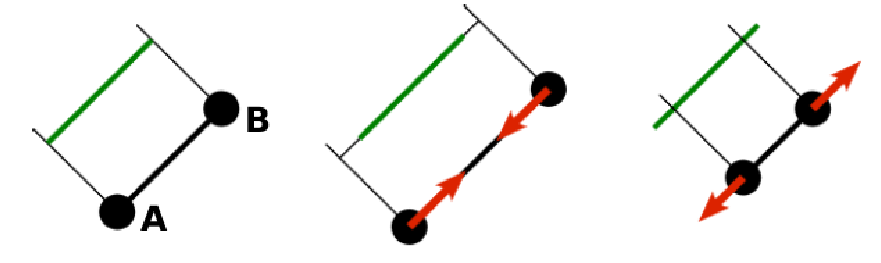
\includegraphics[width=8cm]{figures/stretching.png}
\end{center}
The stretching force acts between two particles and is symmetric. Therefore if an interaction is defined by
\begin{verbatim} 
inter 1 stretching_force 2.0 4.0
\end{verbatim}
then the following two commands
\begin{verbatim} 
part 42 bond 1 43
part 43 bond 1 42
\end{verbatim}
are equivalent.

\subsection{Linear stretching force}
\index{linear stretching force|mainindex}
\index{interactions!linear stretching force|mainindex}

\begin{essyntax}
  inter \var{bondid}
  stretchlin_force
  \var{L^0_{AB}} \var{k_slin}
\end{essyntax}
This type of interaction is available for closed 3D immersed objects as well as 
for 2D sheet flowing in the 3D flow. 

This type of interaction is the linear equivalent of stretching_force. The expressions for the forces are 
the same except $\kappa(\lambda_{AB}) = 1$. 


\subsection{Bending force}
\index{bending force|mainindex}
\index{interactions!bending force|mainindex}

\begin{essyntax}
  inter \var{bondid}
  bending_force
  \var{\theta^0} \var{k_b}
\end{essyntax}

The tendency of an elastic object to maintain the resting shape is governed by 
prescribing the prefered angles between the neighbouring triangles of the mesh. 
This type of interaction is available for closed 3D immersed objects as well as 
for 2D sheet flowing in the 3D flow.


Denote by $\theta^0$ the angle between two triangles in the resting shape. For 
closed immersed objects, you always have to set the inner angle. The deviation 
of this angle $\Delta \theta = \theta - \theta^0$ is computed and defines two 
bending forces for two triangles \var{A_1BC} and \var{A_2BC}
\begin{equation}
\var{F_{bi}(A_iBC)} = \var{k_b}\frac{\Delta \theta}{\theta^0} \var{n_{A_iBC}}
\end{equation}
Here, \var{n_{A_iBC}} is the unit normal vector to the triangle \var{A_iBC}. The 
force \var{F_{bi}(A_iBC)} is assigned to the vertex not belonging to the common 
edge. The opposite force divided by two is assigned to the two vertices lying on 
the common edge. This procedure is done twice, for $\var{i}=1$ and for 
$\var{i}=2$.

\begin{center}
  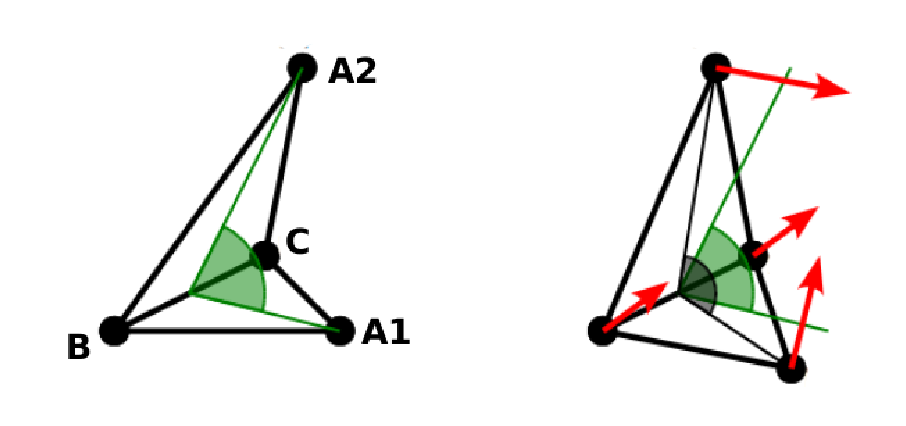
\includegraphics[width=8cm]{figures/bending.png}
\end{center}

Unlike the stretching force the bending force is strictly asymmetric. After 
creating an interaction
\begin{verbatim} 
inter 33 bending_force 0.7 4.0
\end{verbatim}
it is important how the bond is created. Particles need to be mentioned in the 
correct order. Command
\begin{verbatim} 
part 0 bond 33 1 2 3
\end{verbatim}
creates a bond related to the angle between the triangles 012 and 123. The particle 
0 corresponds to point A1, particle 1 to C, particle 2 to B and particle 3 to A2. 
There are two rules that need to be fulfilled:
\begin{itemize}
\item there has to be an edge between particles 1 and 2
\item orientation of the triangle 012, that is the normal vector 
defined as a vector product $01 \times 02$, must point to the inside of the immersed 
object.
\end{itemize}
Notice that also concave objects can be defined. If $\theta_0$ is larger than $\pi$, 
then the inner angle is concave.

\subsection{Local area conservation}
\index{local area conservation|mainindex}
\index{interactions!local area conservation|mainindex}

\begin{essyntax}
  inter \var{bondid}
  area_force_local
  \var{S^0_{ABC}} \var{k_{al}}
\end{essyntax}
This interaction conserves the area of the triangles in the triangulation. This 
type of interaction is available for closed 3D immersed objects as well as for 2D 
sheet flowing in the 3D flow.

The deviation of the triangle surface \var{S_{ABC}} is computed from the triangle 
surface in the resting shape $\Delta \var{S_{ABC}} = \var{S_{ABC}} - \var{S_{ABC}^0}$. 
The area constraint assigns the following  shrinking/expanding force to every vertex 
\begin{equation}
 \var{F_{al}(A)} = -\var{k_{al}}\frac{\Delta \var{S_{ABC}}}{\var{S_{ABC}}}\var{w_{A}}
\end{equation}
where \var{k_{al}}  is the area constraint coefficient, and \var{w_{A}} is the unit 
vector pointing from the centroid of triangle \var{ABC} to the vertex \var{A}. 
Similarly the analogical forces are assigned to \var{B} and \var{C}. This interaction 
is symmetric, therefore after defining the interaction
\begin{verbatim} 
inter 44 area_force_local 0.02 4.0
\end{verbatim}
the following commands are equivalent
\begin{verbatim} 
part 0 bond 44 1 2
part 0 bond 44 2 1
part 1 bond 44 0 2
\end{verbatim}

\subsection{Global area conservation}
\index{global area conservation|mainindex}
\index{interactions!global area conservation|mainindex}

\begin{essyntax}
  inter \var{bondid}
  area_force_global
  \var{S^0} \var{k_{ag}}
\end{essyntax}
This type of interaction is available solely for closed 3D immersed objects.

The conservation of local area is sometimes too restrictive. Denote by \var{S} the 
current surface of the immersed object, by \var{S_0} the surface in the relaxed 
state and define $\Delta \var{S} = \var{S} - \var{S_0}$. The global area conservation 
force is defined as
\begin{equation}
\var{F_{ag}(A)} = - \var{k_{ag}}\frac{\Delta \var{S}}{\var{S}}\var{w_{A}}
\end{equation}
Here, the above mentioned force divided by 3 is added to all three particles.
\begin{center}
  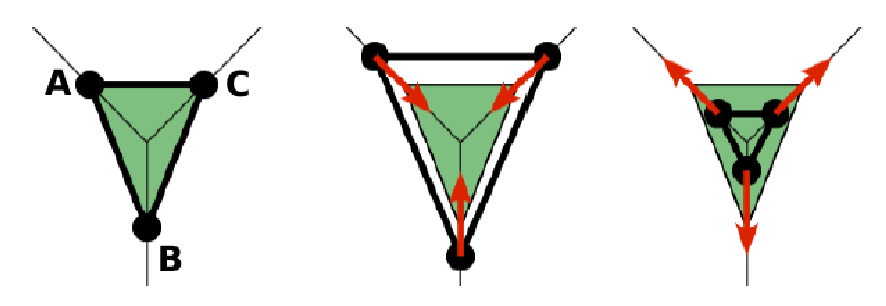
\includegraphics[width=8cm]{figures/arealocal.png}
\end{center}
Again, this interaction is symmetric, as is the area\_{}force\_{}local.

\subsection{Volume conservation}
\index{volume conservation|mainindex}
\index{interactions!volume conservation|mainindex}

\begin{essyntax}
  inter \var{bondid}
  volume_force
  \var{V^0} \var{k_v}
\end{essyntax}
This type of interaction is available solely for closed 3D immersed objects.

The deviation of the objects volume \var{V} is computed from the volume in 
the resting shape $\Delta \var{V} = \var{V} - \var{V^0}$. For each triangle the following 
force is computed
\begin{equation}
\var{F_v(ABC)} = -\var{k_v}\frac{\Delta \var{V}}{\var{V^0}} \var{S_{ABC}}\ \var{n_{ABC}}
\end{equation}
where \var{S_{ABC}} is the area of triangle \var{ABC}, \var{n_{ABC}} is the normal unit 
vector of plane \var{ABC}, and \var{k_v} is the volume constraint coefficient. The volume 
of one immersed object is computed from
\begin{equation}
\var{V} = \sum_{\var{ABC}}\var{S_{ABC}}\ \var{n_{ABC}}\cdot \var{h_{ABC}}
\end{equation}
where the sum is computed over all triangles of the mesh and \var{h_{ABC}} is the normal 
vector from the centroid of triangle \var{ABC} to any plane which does not cross the cell. 
The force \var{F_v(ABC)} is equally distributed to all three vertices $\var{A},\var{B},
\var{C}.$

\begin{center}
  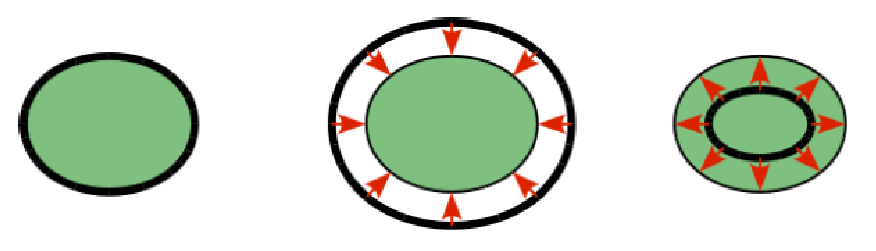
\includegraphics[width=8cm]{figures/volume.png}
\end{center}
This interaction is again symmetric. After the definition of the interaction by 
\begin{verbatim} 
inter 22 volume_force 65.3 3.0
\end{verbatim}
the order of vertices is crucial. By the following command the bonds are defined
\begin{verbatim} 
part 0 bond 22 1 2
\end{verbatim}
Triangle 012 must have correct orientation, that is the normal vector defined by a 
vector product $01\times02$. The orientation must point inside the immersed object.


\section{Bond-angle interactions}
\index{bond-angle interactions|mainindex}
\index{interactions!bond-angle|mainindex}
\label{sec:angle}

\begin{essyntax}
  \variant{1} inter \var{bondid} angle\_harmonic \var{K} \opt{\var{\phi_0}}
  \variant{2} inter \var{bondid} angle\_cosine \var{K} \opt{\var{\phi_0}}
  \variant{3} inter \var{bondid} angle\_cossquare \var{K} \opt{\var{\phi_0}}
  \begin{features}
    \required{BOND_ANGLE}
  \end{features}
\end{essyntax}

This creates a bond type with identificator \var{bondid}
with an angle dependent potential. This potential is defined between
three particles. The particle for which the bond is created, is the
central particle, and the angle $\phi$ between the vectors from this
particle to the two others determines the interaction.  \var{K} is the
bending constant, and the optional parameter $\var{\phi_0}$ is the
equilibirum bond angle in radian ranging from 0 to $\pi$.  If this
parameter is not given, it defaults to $\var{\phi_0} = \pi$, which
corresponds to a stretched configuration. For example, for a bond
defined by
\begin{code}
  part \$p_2 bond 4 \$p_1 \$p_3
\end{code}
the minimal energy configurations are the following:
\begin{center}
  \setlength{\unitlength}{3000sp}
  \begin{picture}(8381,2684)(1570,-5393)
    \thinlines
    \put(2701,-4561){\circle*{450}}
    \put(3601,-4561){\circle*{450}}
    \put(4501,-4561){\circle*{450}}
    \put(7021,-4561){\circle*{450}}
    \put(7921,-4561){\circle*{450}}
    \put(7921,-3661){\circle*{450}}
    \thicklines
    \put(2701,-4561){\line( 1, 0){1800}}
    \put(7021,-4561){\line( 1, 0){900}}
    \put(7921,-4561){\line( 0, 1){900}}
    \put(5761,-2831){\line( 0,-1){2500}}

    \put(2701,-5191){\makebox(0,0)[b]{$p_1$}}
    \put(3601,-5191){\makebox(0,0)[b]{$p_2$}}
    \put(4501,-5191){\makebox(0,0)[b]{$p_3$}}
    \put(7021,-5191){\makebox(0,0)[b]{$p_1$}}
    \put(8371,-3751){\makebox(0,0)[b]{$p_3$}}
    \put(7921,-5191){\makebox(0,0)[b]{$p_2$}}
    \put(8371,-2941){\makebox(0,0)[b]{\keyword{inter 4 angle\var{\_type} 1.0 [expr [PI]/2]}}}
    \put(3601,-2941){\makebox(0,0)[b]{\keyword{inter 4 angle\var{\_type} 1.0 [PI]}}}
  \end{picture}%
\end{center}

For the potential acting between the three particles three variants are possible
\begin{itemize}
\item Harmonic bond angle potential \variant{1}:\\
  A classical harmonic potential,
  \begin{equation}
    V(\phi) = \frac{K}{2} \left(\phi - \phi_0\right)^2.
  \end{equation}
  Unlike the two following variants, this potential has a kink at
  $\phi=\phi_0+\pi$ and accordingly a discontinuity in the force, and should
  therefore be used with caution.
\item Cosine bond angle potential \variant{2}:\\
  \begin{equation}
    V(\alpha) = K \left[1 - \cos(\phi - \phi0)\right]
  \end{equation}
  Around $\phi_0$, this potenial is close to a harmonic one (both are
  $1/2(\phi-\phi_0)^2$ in leading order), but it is periodic and smooth for all
  angles $\phi$.
\item Cosine square bond angle potential \variant{3}:\\
  \begin{equation}
    V(\alpha) = \frac{K}{2} \left[\cos(\phi) - \cos(\phi_0)\right]^2
  \end{equation}
  This form is used for example in the GROMOS96 force field. The potential is
  $1/8(\phi-\phi_0)^4$ around $\phi_0$, and therefore much flatter than the
  two potentials before.
\end{itemize}

\section{Dihedral interactions}
\index{dihedral interactions|mainindex}
\index{interactions!dihedral|mainindex}
\label{sec:dihedral}

\begin{essyntax}
  inter \var{bondid} dihedral \var{n} \var{K} \var{p}
\end{essyntax}

This creates a bond type with identificator \var{bondid}
with a dihedral potential, \ie a four-body-potential. In the following,
let the particle for which the bond is created be particle $p_2$, and
the other bond partners $p_1$, $p_3$, $p_4$, in this order, \ie
\lit{part $p_2$ bond bondid $p_1$ $p_3$ $p_4$}. Then, the
dihedral potential is given by
\begin{equation}
  V(\phi) = \var{K}\left[1 - \cos(\var{n}\phi - \var{p})\right],
\end{equation}
where \var{n} is the multiplicity of the potential (number of minimas)
and can take any integer value (typically from 1 to 6), $p$ is a phase
parameter and \var{K} is the bending constant of the potential. $\phi$
is the dihedral angle between the particles defined by the particle
quadrupel $p_1$, $p_2$, $p_3$ and $p_4$, \ie the angle between the
planes defined by the particle triples $p_1$, $p_2$ and $p_3$ and
$p_2$, $p_3$ and $p_4$:
\begin{center}
  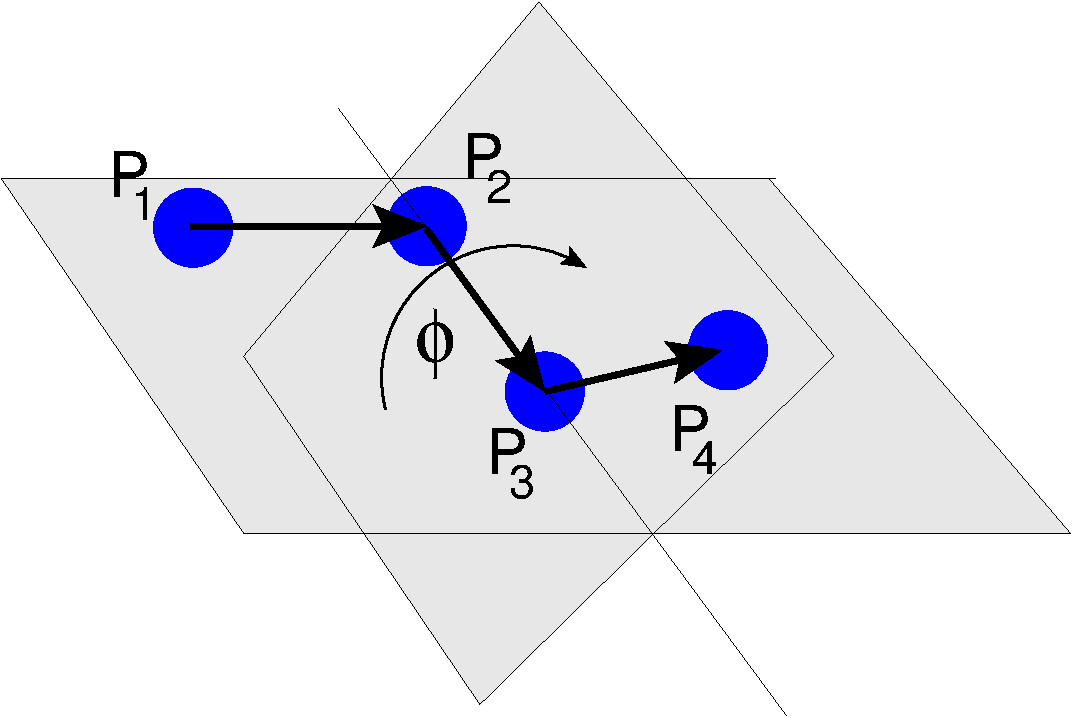
\includegraphics[height=8em]{figures/dihedral-angle}
\end{center}
Together with appropriate Lennard-Jones interactions, this potential
can mimic a large number of atomic torsion potentials.

If you enable the feature OLD_DIHEDRAL, then the old, less
general form of the potential is used:
\begin{equation}
  V(\phi) = \var{K}\left[1 + \var{p}\,\cos(\var{n}\phi)\right],
\end{equation}
where $p$ is rather a phase factor and can only take values $p=\pm 1$.


\section{Coulomb interaction}
\label{sec:inter-electrostatics}
\index{Coulomb interactions|mainindex}
\index{Electrostatic interactions|mainindex}
\index{interactions!Coulomb|mainindex}
\index{interactions!Electrostatic|mainindex}

\begin{essyntax}
  \variant{1} inter coulomb 0.0
  \variant{2} inter coulomb
  \variant{3} inter coulomb \var{parameters}
\end{essyntax}

These commands allow to set up the calculation of the Coulomb
interaction.  The Coulomb (or electrostatic) interaction is defined as
follows.  For a pair of particles at distance $r$ with charges $q_1$
and $q_2$, the interaction is given by
\begin{equation}
  U^C(r)=l_B k_B T\frac{q_1 q_2}{r}.
\end{equation}
where $l_B = e_o^2 / (4 \pi \epsilon k_B T)$ denotes the Bjerrum
length, which measures the strength of the electrostatic interaction.
As a special case, when the internal variable \var{temperature} 
is set to zero, the value of bjerrum length you enter 
is treated as $l_B k_B T$ rather than $l_B$. This occurs when the
thermostat is switched off and \es performs an NVE integration
(see also Section~\ref{sec:thermostat}).

Computing electrostatic interactions is computationally very
expensive.  \es{} features some state-of-the-art algorithms to deal
with these interactions as efficiently as possible, but almost all of
them require some knowledge to use them properly.  Uneducated use can
result in completely unphysical simulations.

Variant \variant{1} disables Coulomb interactions.  Variant
\variant{2} returns the current parameters of the coulomb interaction
as a Tcl-list using the same syntax as used to setup the method, \eg
\begin{tclcode}
  {coulomb 1.0 p3m 7.75 8 5 0.1138 0.0}
  {coulomb epsilon 0.1 n_interpol 32768 mesh_off 0.5 0.5 0.5}
\end{tclcode}

Variant \variant{3} is the generic syntax to set up a specific method
or its parameters, the details of which are described in the following
subsections.  Note that using the electrostatic interaction also
requires assigning charges to the particles.  This is done using the
\texttt{part} command to set the charge \texttt{q}, \eg
\begin{tclcode}
  inter coulomb 1.0 p3m tune accuracy 1e-4
  part 0 q 1.0; part 1 q -1.0
\end{tclcode}

\subsection{Coulomb P3M}
\label{sec:coulomb}
\index{P3M method|mainindex}
\index{interactions!P3M|mainindex}

\begin{essyntax}
  inter coulomb \var{l_B} p3m [gpu] 
  \var{r_\mathrm{cut}} \alt{\var{mesh} \asep \{\var{mesh_x} \var{mesh_y} \var{mesh_z}\}} \var{cao} \var{alpha}
  \begin{features}
    \required{ELECTROSTATICS}
  \end{features}
\end{essyntax}

For this feature to work, you need to have the \texttt{fftw3} library
installed on your system. In \es{}, you can check if it is compiled in
by checking for the feature \texttt{FFTW}.

This command activates the P3M method to compute the electrostatic
interactions between charged particles.  The different parameters are
described in more detail in \cite{deserno98a}.
\begin{description}
\item[\var{[gpu]}]
The optional flag gpu causes the far field portion of p3m to be calculated on the GPU.  It should be noted that this does not always provide significant increase in performance.  Furthermore it computes the far field interactions with only single precision which limits the maximum precision.  Furthermore the algorithm does not work in combination with certain other methods implemented in ESPResSo and only for the case of cubic boxes.
\item[\var{r_\mathrm{cut}}] The real space cutoff as a positive
  floating point number.
\item[\var{mesh}] The number of mesh points, as a single positive
  integer.
\item[\var{mesh_{x,y,z}}] The number of mesh points in x, y and z
  direction. This is relevant for noncubic boxes.
\item[\var{cao}] The \emph{charge-assignment order}, an integer
  between $0$ and $7$.
\item[\var{alpha}] The Ewald parameter as a positive floating point
  number.
\end{description}

Make sure that you know the relevance of the P3M parameters before
using P3M! If you are not sure, read the following references
\cite{ewald21, hockney88, kolafa92, deserno98, deserno98a, deserno00,
  deserno00a, cerda08a}.


\subsubsection{Tuning Coulomb P3M}
\label{ssec:tunep3m}
\begin{essyntax}
  inter coulomb \var{l_B} p3m \alt{tune \asep tunev2} [gpu]
  accuracy \var{accuracy}\\
  \opt{r_cut \var{r_\mathrm{cut}}}
  \opt{mesh \var{mesh}}
  \opt{cao \var{cao}}
  \opt{alpha \var{\alpha}}
  \begin{features}
    \required{ELECTROSTATICS}
  \end{features}
\end{essyntax}

It is not easy to calculate the various parameters of the P3M method
such that the method provides the desired accuracy at maximum speed.
To simplify this, \es{} provides a function to automatically tune the
algorithm.  Note that for this function to work properly, your system
should already contain an initial configuration of charges and the
correct initial box size. Also note that both provided tuning
algorithms work very well on homogenous charge distributions, but
might not achieve the requested precision for highly inhomogenous or
symmetric systems. For example, because of the nature of the P3M
algorithm, systems are problematic where most charges are placed in
one plane, one small region, or on a regular grid.

The function employs the analytical expression of the error estimate
for the P3M method \cite{hockney88} and its real space error
\cite{kolafa92} to obtain sets of parameters that yield the desired
accuracy, then it measures how long it takes to compute the coulomb
interaction using these parameter sets and chooses the set with the
shortest run time.

The function will only automatically tune those parameters that are
not set to a predetermined value using the optional parameters of the
tuning command.

The two tuning methods follow different methods for determining the
optimal parameters. While the \keyword{tune} version tests different
values on a grid in the parameter space, the \keyword{tunev2} version
uses a bisection to determine the optimal parameters.  In general, for
small systems the \keyword{tune} version is faster, while for large
systems \keyword{tunev2} is faster. The results of \keyword{tunev2}
are always at least as good as the parameters from the \keyword{tune}
version, and normally the obtained accuracy is much closer to the
desired value.

During execution the tuning routines report the tested parameter sets,
the corresponding k-space and real-space errors and the timings needed
for force calculations (the setmd variable \var{timings} controls the
number of test force calculations).  Since the error depends on
\var{r_\mathrm{cut}}/\var{box\_l} and \var{\alpha}\var{box\_l} the
output is given in these units.

Note that the previous setting of \var{r_\mathrm{cut}}, \var{cao} and
\var{mesh} will be remembered.  If you want to retune your
electrostatics, \eg after a major system change, you should use
\begin{code}
  inter coulomb \var{l_B} p3m tune accuracy \var{acc} r_cut 0 mesh 0 cao 0
\end{code}

\subsubsection{Additional P3M parameters}

\begin{essyntax}
  inter coulomb \opt{\lit{epsilon} \alt{\lit{metallic} \asep \var{epsilon}}}
  \opt{\lit{n_interpol} \var{points}} \opt{\lit{mesh_off} \var{xoff}
    \var{yoff} \var{zoff}}
\end{essyntax}

Once P3M algorithm has been set up, it is possible to set some
additional P3M parameters with this command.  The different parameters
have the following meaning:
\begin{description}
\item[\lit{epsilon} \var{epsilon}] The dielectric constant of the
  surrounding medium, metallic (\ie infinity) or some finite positive
  number.  Defaults to \lit{metallic}.
\item[\lit{n_interpol} \var{n_interpol}] Number of interpolation
  points for the charge assignment function.  When this is set to $0$,
  interpolation is turned off and the function is computed directly.
  Defaults to $32768$.
\item[\lit{mesh_off} \var{mesh_off}] Offset of the first mesh point
  from the lower left corner of the simulation box in units of the
  mesh constant. Defaults to \codebox{{0.5 0.5 0.5}}.
\end{description}


\subsection{Debye-H\"uckel potential}
\index{Debye-H\"uckel potential|mainindex}
\index{interactions!Debye-H\"uckel|mainindex}

\begin{essyntax}
  inter coulomb \var{l_B} dh \var{\kappa} \var{r_\mathrm{cut}}
  \begin{features}
    \required{ELECTROSTATICS}
  \end{features}
\end{essyntax}

Defines the electrostatic potential by
\begin{equation}
  U^{C-DH} = l_B k_B T \frac{q_1 q_2 exp(-\kappa r)}{r}\quad \mathrm{for}\quad r<r_{\mathrm{cut}}
\end{equation}

The Debye-H\"uckel potential is an approximate method for calculating
electrostatic interactions, but technically it is treated as other
short-ranged non-bonding potentials. For $r>r_{\mathrm cut}$ it is set 
to zero which introduces a step in energy. Therefore, it introduces
fluctuations in energy.

For $\kappa = 0$, this corresponds to the plain coulomb potential.

\subsection{MMM2D}
\index{MMM2D method|mainindex}
\index{interactions!MMM2D|mainindex}

\begin{citebox}
  Please cite~\citewbibkey{mmm2d} when using MMM2D, and
  \citewbibkey{icmmm2d} when using dielectric interfaces.
\end{citebox}


\begin{essyntax}
 inter coulomb \var{l_B} mmm2d \var{maximal\_pairwise\_error}
 \opt{\var{fixed\_far\_cutoff}}
 \opt{dielectric \var{\epsilon_t} \var{\epsilon_m} \var{\epsilon_b}}
 \opt{dielectric-contrasts \var{\Delta_t} \var{\Delta_b}}
  \begin{features}
    \required{ELECTROSTATICS}
  \end{features}
\end{essyntax}
MMM2D coulomb method for systems with periodicity 1 1 0. Needs the
layered cell system. The performance of the method depends on the
number of slices of the cell system, which has to be tuned manually.
It is automatically ensured that the maximal pairwise error is smaller
than the given bound. The far cutoff setting should only be used for
testing reasons, otherwise you are more safe with the automatical
tuning. If you even don't know what it is, do not even think of
touching the far cutoff. For details on the MMM family of algorithms,
refer to appendix \vref{chap:mmm}.

The last two, mutually exclusive arguments ``dielectric'' and
``dielectric-constants'' allow to specify dielectric contrasts at the
upper and lower boundaries of the simulation box. The first form
specifies the respective dielectric constants in the media, which
however is only used to calculate the contrasts. That is, specifying 
$\epsilon_t=\epsilon_m=\epsilon_b=\text{const}$ is always identical to
$\epsilon_t=\epsilon_m=\epsilon_b=1$. The second form specifies only
the dielectric contrasts at the boundaries, that is
$\Delta_t=\frac{\epsilon_m-\epsilon_t}{\epsilon_m+\epsilon_t}$ and
$\Delta_b=\frac{\epsilon_m-\epsilon_b}{\epsilon_m+\epsilon_b}$. Using
this form allows to choose $\Delta_{t/b}=-1$, corresponding to
metallic boundary conditions.

\subsection{MMM1D}
\index{MMM1D method|mainindex}
\index{interactions!MMM1D|mainindex}

\begin{citebox}
  Please cite~\citewbibkey{mmm1d} when using MMM1D.
\end{citebox}

\begin{essyntax}
  \variant{1}
  inter coulomb \var{l_B} mmm1d \var{switch\_radius}
  \opt{\var{bessel\_cutoff}} \var{maximal\_pairwise\_error}

  \variant{2}
  inter coulomb \var{l_B} mmm1d tune \var{maximal\_pairwise\_error}
  \begin{features}
    \required{ELECTROSTATICS}
  \end{features}
\end{essyntax}
MMM1D coulomb method for systems with periodicity 0 0 1. Needs the
nsquared cell system (see section \vref{sec:cell-systems}). The first
form sets parameters manually. The switch radius determines at which
xy-distance the force calculation switches from the near to the far
formula. If the Bessel cutoff is not explicitly given, it is
determined from the maximal pairwise error, otherwise this error only
counts for the near formula. The second, tuning form just takes the
maximal pairwise error and tries out a lot of switching radii to find
out the fastest one. If this takes too long, you can change the value
of the setmd variable \keyword{timings}, which controls the number of
test force calculations. For details on the MMM family of algorithms,
refer to appendix \vref{chap:mmm}.

\subsection{Maxwell Equation Molecular Dynamics (MEMD)}
\index{Maggs method|mainindex}
\index{Maxwell Equation Molecular Dynamics|mainindex}
\index{MEMD|mainindex}
\index{interactions!Maggs method|mainindex}
\index{interactions!MEMD|mainindex}

\begin{essyntax}
  inter coulomb \var{l_B}
  memd \var{f\_mass} \var{mesh} \opt{epsilon \var{\varepsilon_{\infty}}}
  \begin{features}
    \required{ELECTROSTATICS}
  \end{features}
\end{essyntax}

This is an implementation of the instantaneous 1/r Coulomb interaction
\begin{equation}
  U = l_B k_B T \frac{q_1 q_2}{r}
\end{equation}
as the potential of mean force between charges which are dynamically
coupled to a local electromagnetic field.

The algorithm currently works with the following constraints:

\begin{itemize}
  \item cellsystem has to be domain decomposition but \emph{without}
    Verlet lists!
  \item system has to be periodic in three dimensions.
\end{itemize}

\begin{arguments}
\item[\var{f\_mass}] is the mass of the field degree of freedom and equals
  to the square root of the inverted speed of light.
\item[\var{mesh}] is the number of mesh points for the interpolation
  of the electromagnetic field in one dimension.
\item[\var{\varepsilon_{\infty}}] is the background dielectric
  permittivity at infinity. This defaults to metallic boundary
  conditions, to match the results of P3M.
\end{arguments}

The arising self-interactions are treated with a modified version of
the exact solution of the lattice Green's function for the
problem.

Currently, forces have large errors for two particles within the same
lattice cube. This may be fixed in future development, but right now
leads to the following rule of thumb for the parameter choices:

\begin{itemize}
  \item The lattice should be of the size of your particle size
    (i.e. the lennard jones epsilon). That means: $\text{mesh} \approx
    \text{box\_l} / \text{lj\_sigma}$
  \item The integration timestep should be in a range where no
    particle moves more than one lattice box (i.e. lennard jones
    sigma) per timestep.
  \item The speed of light should satisfy the stability criterion
    $c\ll a/dt$, where $a$ is the lattice spacing and $dt$ is the
    timestep. For the second parameter, this means $\text{f\_mass} \gg
    dt^2/a^2$.
\end{itemize}

The main error of the MEMD algorithm stems from the lattice
interpolation and is proportional to the lattice size in three
dimensions, which means $\Delta_\text{lattice} \propto a^3$.

Without derivation here, the algorithmis error is proportional to
$1/c^2$, where $c$ is the adjustable speed of light. From the
stability criterion, this yields

\begin{equation}
\Delta_\text{maggs} = A\cdot a^3 + B\cdot dt^2/a^2
%\label{eq:maggserror}
\end{equation}

This means that increasing the lattice will help the algorithmic
error, as we can tune the speed of light to a higher value. At the
same time, it increases the interpolation error at an even higher
rate. Therefore, momentarily it is advisable to choose the lattice
with a rather fine mesh of the size of the particles. As a rule of
thumb, the error will then be less than $10^{-5}$ for the particle
force.

For a more detailed description of the algorithm, see
appendix~\vref{sec:MEMD} or the publications~\cite{maggs02a,
  pasichnyk04a}.

\subsubsection{Spatially varying dielectrics with MEMD}
\index{Dielectric interfaces}
\label{sec:dielectric-memd}

Since MEMD is a purely local algorithm, one can apply local changes
to some properties and the propagation of the Coulomb force is still
valid. In particular, it is possible to arbitrarily select the
dielectric permittivity on each site of the interpolating lattice.

\begin{essyntax}
  inter coulomb \var{l_B}
  memd localeps node \var{node\_x} \var{node\_y} \var{node\_z}
  dir \var{X/Y/Z} eps \var{\varepsilon}
  \begin{features}
    \required{ELECTROSTATICS}
  \end{features}
\end{essyntax}

The keyword \keyword{localeps} after the \keyword{inter coulomb}
command offers the possibility to assign any value of $\varepsilon$
to any lattice site.

\begin{arguments}
\item[\var{l_B}] is the bjerrum length of the background. It defines
	the reference value $\varepsilon_\text{bg}$ via the formula 
	\eqref{eq:bjerrum-length}. This is a global variable.
\item[\var{node\_x}] is the index of the node in $x$ direction that
	should be changed
\item[\var{node\_y}] is the index of the node in $y$ direction that
	should be changed
\item[\var{node\_z}] is the index of the node in $z$ direction that
	should be changed
\item[\var{X/Y/Z}] is the direction in which the lattice site to be
	changed is pointing. Has to be one of the three (X, Y or Z).
\item[\var{\varepsilon}] is the relative permittivity change in
	respect to the background permittivity set by the parameter
	\var{l_B}.
\end{arguments}

The permittivity on each lattice site is set relatively. By defining
the (global) bjerrum length of the system, the reference
permittivity~$\varepsilon$ is fixed via the formula

\begin{equation}
l_B = e^2 / (4 \pi \varepsilon k_B T)
\label{eq:bjerrum-length}
\end{equation}

The local changes of $\varepsilon$ are in reference to this value
and can be seen as a spatially dependent prefactor to this epsilon.
If left unchanged, this prefactor is $1.0$ for every site by
default.

\subsection{Electrostatic Layer Correction (ELC)}
\index{ELC method|mainindex}
\index{interactions!ELC method|mainindex}

\begin{citebox}
  Please cite~\citewbibkey{elc} when using ELC, and in addition
  \citewbibkey{icelc} if you use dielectric interfaces.
\end{citebox}

\begin{essyntax}
  inter coulomb elc \var{maximal\_pairwise\_error} \var{gap\_size}
  \opt{\var{far\_cutoff}}
  \opt{noneutralization}
  \opt{dielectric \var{\epsilon_t} \var{\epsilon_m} \var{\epsilon_b}}
  \opt{dielectric-contrasts \var{\Delta_t} \var{\Delta_b}}
  \begin{features}
    \required{ELECTROSTATICS}
  \end{features}
\end{essyntax}
This is a special procedure that converts a 3d method, to a 2d method,
in computational order N. Currently, it only supports P3M. This means,
that you will first have to set up the P3M algorithm (via
\texttt{inter coulomb p3m \var{params}}) before using ELC.  The
algorithm is definitely faster than MMM2D for larger numbers of
particles ($>400$ at reasonable accuracy requirements). The maximal
pairwise error \var{maximal\_pairwise\_error} sets the LUB error of
the force between any two charges without prefactors (see the
papers). The algorithm tries to find parameters to meet this LUB
requirements or will throw an error if there are none.

The gap size \var{gap\_size} gives the height of the empty region
between the system box and the neighboring artificial images (again,
see the paper).  \es does not make sure that the gap is actually
empty, this is the users responsibility. The method will compute fine
of the condition is not fulfilled, however, the error bound will not
be reached. Therefore you should really make sure that the gap region
is empty (e. g. by constraints).

The setting of the far cutoff \var{far\_cutoff} is only intended for
testing and allows to directly set the cutoff. In this case, the
maximal pairwise error is ignored. The periodicity has to be set to
\texttt{1 1 1} still, and the 3d method has to be set to epsilon
metallic, i.e.  metallic boundary conditions. For details, see
appendix \vref{chap:mmm}.

By default, ELC just as P3M adds a homogeneous neutralizing background
to the system in case of a net charge. However, unlike in three
dimensions, this background adds a parabolic potential across the
slab~\cite{ballenegger09a}. Therefore, under normal circumstance, you
will probably want to disable the neutralization using
\opt{noneutralization}. This corresponds then to a formal
regularization of the forces and energies~\cite{ballenegger09a}. Also,
if you add neutralizing walls explicitely as constraints, you have to
disable the neutralization.

The dielectric contrast features work exactly the same as for MMM2D,
see the documentation above.

Make sure that you read the papers on ELC (\cite{elc,icelc})
before using it.

\subsection{Dielectric interfaces with the ICC$\star$ algorithm}
\index{ICC$\star$|mainindex}
\index{Dielectric interfaces}
\newescommand{iccp3m}

\begin{essyntax}
  iccp3m \var{n\_induced\_charges} 
  convergence \var{convergence\_criterion}
  areas \var{areas}
  normals \var{normals}
  sigmas \var{sigmas}
  epsilons \var{epsilons}
  \opt{eps\_out \var{eps\_out} }
  \opt{relax \var{relaxation\_parameter} }
  \opt{max\_iterations \var{max\_iterations} }
  \opt{ext\_field \var{ext\_field}}
  \begin{features}
    \required{ELECTROSTATICS}
  \end{features}
\end{essyntax}

The ICC$\star$ algorithm allows to take into account arbitrarily
shaped dielectric interfaces.  This is done by iterating the charge on
the particles with the ids 0 to \var{n\_induced\_particles-1} until
the correctly represent the influence of the dielectric
discontinuity. It relies on a coulomb solver that is already
initialized. This Coulomb solver can be P3M, P3M+ELC, MMM2D or MMM1D.
As most of the times, ICC$\star$ will be used with P3M the
corresponding command is called \keyword{iccp3m}.

Please make sure to read the corresponding articles,
mainly\cite{espresso2, tyagi10a, kesselheim11a} before using it.

The particles with ids 0 to \var{n\_induced\_particles-1} are treated
as iterated particles by ICC$\star$.  The constitute the dielectric
interface and should be fixed in space. The parameters \var{areas} and
\var{epsilons} are Tcl lists containing one floating point number
describing each surface elements area and dielectric
constant. \var{sigmas} allows to take into account a (bare) charge
density, thus a surface charge density in absence of any charge
induction. \var{normals} is a Tcl list of Tcl lists with three
floating point numbers describing the outward pointing normal vectors
for every surface element.  The parameter \var{convergence\_criterion}
allows to specify the accuracy of the iteration. It corresponds to the
maximum relative change of any of the interface particle's
charge. After \var{max\_iterations} the iteration stops anyways. The
dielectric constant in bulk, i.~e. outside the dielectric walls is
specified by \var{eps\_out}. A homogenous electric field can be added
to the calculation of dielectric boundary forces by specifying it in
the parameter \var{ext\_field}.

\subsubsection{Quick setup of dielectric interfaces}
\index{Dielectric interfaces}
\newescommand{dielectric}

\begin{essyntax}
  \variant{1} dielectric sphere center \var{cx} \var{cy} \var{cz} radius \var{r} res \var{res} 
  \variant{2} dielectric wall normal \var{nx} \var{ny} \var{nz} dist \var{d} res \var{res}
  \variant{3} dielectric cylinder  center \var{cx} \var{cy} \var{cz} axis \var{ax} \var{ay} \var{az} radius \var{r} direction \var{d} 
  \variant{4} dielectric pore center \var{cx} \var{cy} \var{cz}  axis \var{ax} \var{ay} \var{az} radius \var{r} length \var {l} smoothing\_radius \var{rs} res \var{res}
  \variant{5} dielectric slitpore pore_mouth \var{z} \
             channel_width \var{c} \
             pore_width \var{w} \
             pore_length \var{l} \
             upper_smoothing_radius \var{us} \
             lower_smoothing_radius \var{ls} 

\end{essyntax}

The command \keyword{dielectric} allows to conveniently create
dielectric interfaces similar to the constraint and the lbboundary
command. Currently the creation of spherical, cylindrical and planar
geometries as well as a pore and slitpore geometry is supported.
Please check the documentation of the corresponding constraint for the detailed geometry.
It is implemented
in Tcl and places particles in the right positions and adds the
correct values to the global Tcl variables \var{icc\_areas}
\var{icc\_normals} \var{icc\_sigmas} \var{icc\_epsilons} and increases
the global Tcl variable var{n\_induced\_charges}. Thus after setting
up the shapes, it is still necessary to register them by calling
\keyword{iccp3m}, usually in the following way:
\begin{code}
  iccp3m \$n\_induced\_charges epsilons \$icc\_epsilons normals \\ 
  \$icc\_normals areas \$icc\_areas sigmas \$icc\_sigmas
\end{code}

\section{Dipolar interaction}
\label{sec:inter-dipolar}
\index{Dipolar interactions|mainindex}
\index{Magnetostatic interactions|mainindex}
\index{interactions!Dipolar|mainindex}
\index{interactions!Magnetostatic|mainindex}

\begin{essyntax}
  \variant{1} inter magnetic 0.0
  \variant{2} inter magnetic
  \variant{3} inter magnetic \var{parameters}
\end{essyntax}

These commands can be used to set up magnetostatic interactions, which
is defined as follows:
\begin{equation}
  U^{D-P3M}(\vec{r}) = l_{B} k_B T \left( \frac{(\vec{\mu}_i \cdot \vec{\mu}_j)}{r^3} 
  - \frac{3  (\vec{\mu}_i \cdot \vec{r})  (\vec{\mu}_j \cdot \vec{r}) }{r^5} \right)
\end{equation}
where $r=|\vec{r}|$.

$l_{B}$ is a dimensionless parameter similar to the Bjerrum length in
electrostatics which helps to tune the effect of the medium on the
magnetic interaction between two magnetic dipoles.

Computing magnetostatic interactions is computationally very
expensive.  \es{} features some state-of-the-art algorithms to deal
with these interactions as efficiently as possible, but almost all of
them require some knowledge to use them properly.  Uneducated use can
result in completely unphysical simulations.

The commands above work as their couterparts for the electrostatic
interactions (see section \vref{sec:coulomb}).  Variant \variant{1}
disables dipolar interactions.  Variant \variant{2} returns the
current parameters of the dipolar interaction as a Tcl-list using the
same syntax as used to setup the method, \eg
\begin{tclcode}
  {coulomb 1.0 p3m 7.75 8 5 0.1138 0.0}
  {coulomb epsilon 0.1 n_interpol 32768 mesh_off 0.5 0.5 0.5}
\end{tclcode}

Variant \variant{3} is the generic syntax to set up a specific method
or its parameters, the details of which are described in the following
subsections.  Note that using the magnetostatic interaction also
requires assigning dipole moments to the particles.  This is done
using the \texttt{part} command to set the dipole moment \texttt{dip},
\eg
\begin{tclcode}
  inter coulomb 1.0 p3m tune accuracy 1e-4
  part 0 dip 1 0 0; part 1 dip 0 0 1
\end{tclcode}

\subsection{Dipolar P3M}

\begin{essyntax}
  inter magnetic \var{l_B} p3m 
  \var{r_\mathrm{cut}} \var{mesh} \var{cao} \var{alpha}
  \begin{features}
    \required{DIPOLES}
  \end{features}
\end{essyntax}

This command activates the P3M method to compute the dipolar
interactions between charged particles.  The different parameters are
described in more detail in \cite{cerda08a}.
\begin{description}
\item[\var{r_\mathrm{cut}}] The real space cutoff as a positive
  floating point number.
\item[\var{mesh}] The number of mesh points, as a single positive
  integer.
\item[\var{cao}] The \emph{charge-assignment order}, an integer
  between $0$ and $7$.
\item[\var{alpha}] The Ewald parameter as a positive floating point
  number.
\end{description}

Make sure that you know the relevance of the P3M parameters before
using P3M! If you are not sure, read the following references
\cite{ewald21, hockney88, kolafa92, deserno98, deserno98a, deserno00,
  deserno00a}.

Note that dipolar P3M does not work with non-cubic boxes.

\subsubsection{Tuning dipolar P3M}
\begin{essyntax}
  inter magnetic \var{l_B} p3m \alt{tune \asep tunev2}
  accuracy \var{accuracy}\\
  \opt{r_cut \var{r_\mathrm{cut}}} \opt{mesh \var{mesh}} \opt{cao
    \var{cao}} \opt{alpha \var{\alpha}}
  \begin{features}
    \required{DIPOLES}
  \end{features}
\end{essyntax}

Tuning dipolar P3M works exactly as tuning Coulomb P3M.  Therefore,
for details on how to tune the algorothm, refer to the documentation
of Coulomb P3M (see section \vref{ssec:tunep3m}).

For the magnetic case, the expressions of the error estimate are given
in \cite{cerda08a}.

\subsection{Dipolar Layer Correction (DLC)}
\index{DLC method|mainindex}
\index{interactions!DLC method|mainindex}

\begin{essyntax}
  inter magnetic mdlc \var{accuracy} \var{gap\_size}
  \opt{\var{far\_cutoff}}
  \begin{features}
    \required{DIPOLES}
  \end{features}
\end{essyntax}

Like ELC but applied to the case of magnetic dipoles, but here the
accuracy is the one you wish for computing the energy.
\var{far_cutoff} is set to a value that, assuming all dipoles to be as
larger as the largest of the dipoles in the system, the error for the
energy would be smaller thant the value given by accuracy. At this
moment you cannot compute the accuracy for the forces, or torques,
nonetheless, usually you will have an error for forces and torques
smaller than for energies. Thus, the error for the energies is an
upper boundary to all errors in the calculations.

At present, the program assumes that the gap without particles is
along the z-direction.  The gap-size is the length along the
z-direction of the volume where particles are not allowed to enter.

As a reference for the DLC method, see \cite{brodka04a}.

\subsection{Dipolar all-with-all and no replicas (DAWAANR)}
\index{DAWAANR method|mainindex}
\index{interactions!DAWAANR method|mainindex}

\begin{essyntax}
  inter magnetic \var{l_{B}} dawaanr
  \begin{features}
    \required{DIPOLES}
  \end{features}
\end{essyntax}

This interaction calculates energies and forces between dipoles by
explicitly summing over all pairs.  For the directions in which the
system is periodic (as defined by \texttt{setmd periodic}), it applies
the minimum image convention, i.e. the interaction is effectively cut
off at half a box length.

In periodic systems, this method should only be used if it is not possible to use dipolar P3M or
DLC, because those methods have a far better accuracy and are much faster.
In a non-periodic system, the DAWAANR-method gives the exact result.

\subsection{Magnetic Dipolar Direct Sum (MDDS)}
\index{MDDS method|mainindex}
\index{interactions!MDDS method|mainindex}

\begin{essyntax}
  inter magnetic \var{l_{B}} mdds n\_cut \var{value\_n\_cut}
  \begin{features}
    \required{DIPOLES}
    \required{MAGNETIC_DIPOLAR_DIRECT_SUM}
  \end{features}
\end{essyntax}

The command enables the ``magnetic dipolar direct sum''.  The
dipole-dipole interaction is computed by explicitly summing over all
pairs. If the system is periodic in one or more directions, the
interactions with further \var{value\_n\_cut} replicas of the system
in all periodic directions is explicitly computed.

As it is very slow, this method is not intended to do simulations,
but rather to check the results you get from more efficient methods
like P3M.
  
\section{Special interaction commands}
\label{sec:inter-other}

\subsection{Tunable-slip boundary interaction}\label{sec:tunableSlip}
\index{Tunable-slip boundary interaction|mainindex}
\index{interactions!Tunable-slip boundary interactions|mainindex}
\begin{essyntax}
  inter \var{type1} \var{type2}
  tunable_slip \var{T} \var{\gamma_L} \var{r_\mathrm{cut}} \var{\delta t}
  \var{v_x} \var{v_y} \var{v_z}
  \begin{features}
    \required{TUNABLE_SLIP}
  \end{features}
\end{essyntax}
Simulating microchannel flow phenomena like the Plane Poiseuille and
the Plane Couette Flow require accurate boundary conditions. There are
two main boundary conditions in use:

\begin{enumerate} 
\item \emph{slip boundary condition} which means that the flow
  velocity at the the hydrodynamic boundaries is zero.
\item \emph{partial-slip boundary condition} which means that the flow 
  velocity at the hydrodynamic boundaries does not vanish.
\end{enumerate}

In recent years, experiments have indicated that the no-slip boundary
condition is indeed usually not valid on the micrometer
scale. Instead, it has to be replaced by the \emph{partial-slip
  boundary condition}
\begin{displaymath}
\delta_B \; \; \partial_\mathbf{n} v_{\parallel} \rVert_{\mathbf{r}_B} =
v_{\parallel} \rVert_{\mathbf{r}_B},
\end{displaymath}
where $v_{\parallel}$ denotes the tangential component of the velocity
and $\partial_\mathbf{n} v_{\parallel}$ its spatial derivative normal
to the surface, both evaluated at the position $\mathbf{r}_B$ of the
so-called \emph{hydrodynamic boundary}.  This boundary condition is
characterized by two effective parameters, namely (i) the slip length
$\delta_B$ and (ii) the hydrodynamic boundary $\mathbf{r}_B$.

Within the approach of the tunable-slip boundary interactions it is
possible to tune the slip length systematically from full-slip to
no-slip.  A coordinate-dependent Langevin-equation describes a viscous
layer in the vicinity of the channel walls which exerts an additional
friction on the fluid particles.  \var{T} is the temperature,
\var{\gamma_L} the friction coefficient and \var{r_\mathrm{cut}} is
the cut-off radius of this layer. \var{\delta t} is the timestep of
the integration scheme. With \var{v_x} \var{v_y} and \var{v_z} it is
possible to give the layer a reference velocity to create a Plane
Couette Flow.  Make sure that the cutoff radius \var{r_\mathrm{cut}}
is larger than the cutoff radius of the constraint Lennard-Jones
interactions. Otherwise there is no possibility that the particles
feel the viscous layer.

This method was tested for Dissipative Particle Dynamics but it is
intended for mesoscopic simulation methods in general. Note, that to
use tunable-slip boundary interactions you have to apply \textbf{two}
plane cell constraints with Lennard-Jones in addition to the
tunable-slip interaction. Make sure that the cutoff radius
\var{r_\mathrm{cut}} is larger than the cutoff radius of the
constraint Lennard-Jones interactions. Otherwise there is no
possibility that the particles feel the viscous layer.  Please read
reference \cite{smiatek08a} before using this interaction.

\subsection{DPD interaction}\label{sec:DPDinter}
\index{DPD interaction|mainindex}
\index{interactions!DPD|mainindex}
\index{DPD}

\begin{essyntax}
  inter \var{type1} \var{type2} inter_dpd \var{gamma} \var{r\_cut} \var{wf}  \var{tgamma} \var{tr\_cut} \var{twf}
  \begin{features}
    \required{INTER_DPD}
  \end{features}
\end{essyntax}

This is a special interaction that is to be used in conjunction with
the Dissipative Particle Dynamics algorithm \ref{sec:DPD} when the
\feature{INTER_DPD} implementation is used. The parameters correspond
to the parameters of the DPD thermostat \vref{sec:DPDinter}, but can
be set individually for the different interactions.

\subsection{Fixing the center of mass}
\begin{essyntax}
  inter \var{typeid1} \var{typeid1} comfixed \var{flag}
  \begin{features}
    \required{COMFIXED}
  \end{features}
\end{essyntax}
This interaction type applies a constraint on particles of type
\var{typeid1} such that during the integration the center of mass of
these particles is fixed. This is accomplished as follows: The sum of
all the forces acting on particles of type \var{typeid1} are
calculated. These include all the forces due to other interaction
types and also the thermostat. Next a force equal in magnitude, but in
the opposite direction is applied to all the particles. This force is
divided on the particles of type \var{typeid1} relative to
their respective mass. Under periodic boundary conditions, this fixes
the itinerant center of mass, that is, the one obtained from the
unfolded coordinates.

Note that the syntax of the
declaration of comfixed interaction requires the same particle type to
be input twice. If different particle types are given in the input,
the program exits with an error message. \var{flag} can be set to 1
(which turns on the interaction) or 0 (to turn off the interaction).


Since the necessary communication is lacking at present, this interaction
only works on a single node.

\subsection{Pulling particles apart}
\begin{essyntax}
  inter \var{typeid1} \var{typeid2}
  comforce \var{flag} \var{dir} \var{force} \var{fratio}
  \begin{features}
    \required{COMFORCE}
  \end{features}
\end{essyntax}
The comforce interaction type enables one to pull away particle groups
of two different types. It is mainly designed for pulling experiments
on bundles. Within a bundle of molecules of type number \var{typeid1}
lets mark one molecule as of type \var{typeid2}. Using comforce one
can apply a force such that t2 can be pulled away from the bundle. The
\var{comforce_flag} is set to 1 to turn on the interaction, and to 0
otherwise. The pulling can be done in two different directions. Either
parallel to the major axis of the bundle ($\var{dir} = 0$) or
perpendicular to the major axis of the bundle ($\var{dir} = 1$).
\var{force} is used to set the magnitude of the force.  \var{fratio}
is used to set the ratio of the force applied on particles of
\var{typeid1} vs. \var{typeid2}. This is useful if one has to keep the
total applied force on the bundle and on the target molecule the same.
A force of magnitude \var{force} is applied on \var{typeid2}
particles, and a force of magnitude (\var{force} * \var{fratio}) is
applied on \var{typeid1} particles.

\subsection{Capping the force during warmup}
\label{sec:forcecap}

\begin{essyntax}
  inter forcecap \alt{\var{F_\mathrm{max}} \asep individual}
\end{essyntax}

Non-bonded interactions are often used to model the hard core
repulsion between particles. Most of the potentials in the section are
therefore singular at zero distance, and forces usually become very
large for distances below the particle size. This is not a problem
during the simulation, as particles will simply avoid overlapping.
However, creating an initial dense random configuration without
overlap is often difficult.

By artificially capping the forces, it is possible to simulate a
system with overlaps. By gradually raising the cap value
\var{F_\mathrm{max}}, possible overlaps become unfavorable, and the
system equilibrates to a overlap free configuration.

This command will cap the force to \var{F_\mathrm{\var{max}}}, \ie for
particle distances which would lead to larger forces than
\var{F_\mathrm{max}}, the force remains at \var{F_\mathrm{max}}.
Accordingly, the potential is replaced by $r \var{F_\mathrm{max}}$.
Particles placed exactly on top of each other will be subject to a
force of magnitude \var{F_\mathrm{max}} along the first coordinate axis.

The force capping is switched off by setting $\var{F_\mathrm{max}}=0$.
Note that force capping always applies to all Lennard-Jones, tabulated,
Morse and Buckingham interactions regardless of the particle types.

If instead of a force capping value, the string ``individual'' is
given, the force capping can be set individually for each
interaction. The capping radius is in this case not derived from the
potential parameters, but is given by an additional signal floating
point parameter to the interaction.

%%% Local Variables:
%%% mode: latex
%%% TeX-master: "ug"
%%% End:
